% !TeX program = xelatex
% !Mode:: "TeX:UTF-8"
%%  本模板推荐以下方式编译: xelatex
%%     1. 文件默认的编码为 UTF-8 对于windows,请选用支持UTF-8编码的编辑器。

%%   2. 若是模板有什么问题,请及时与我们取得联系,Email:latexstudio@qq.com。

%%   3. 可以到  https://ask.latexstudio.net 提问
%%   4. 请安装 最新版本的 TeXLive 地址:
%%   http://mirrors.ctan.org/systems/texlive/Images/texlive.iso

\documentclass[12pt,a4paper]{nmmcm}
\usepackage{ctex}
\usepackage{graphicx}
\usepackage{booktabs,colortbl}
\usepackage{xcolor}
\usepackage{tikz}
\usepackage{indentfirst}
\mcmsetup{CTeX = true,
        tcn ={\xiaowuhao 2024030125260 }, problem = C,
        sheet = true, titleinsheet = false, keywordsinsheet = true,
        titlepage = true, abstract = true}
\usepackage{xurl}
\setmainfont[
    Path=fonts/TimesNewRoman/,
    UprightFont = *-Regular,
    BoldFont = *-Bold,
    ItalicFont = *-Italic,
    BoldItalicFont = *-Bold-Italic
]{TimesNewRoman}
\setmonofont[
    Path=fonts/UbuntuMono/,
    UprightFont = *-Regular,
    BoldFont = *-Bold,
    ItalicFont = *-Italic,
    BoldItalicFont = *-Bold-Italic
]{UbuntuMono}
\usepackage{lipsum}

\usepackage{paralist}
\let\itemize\compactitem
\let\enditemize\endcompactitem
\let\enumerate\compactenum
\let\endenumerate\endcompactenum
\let\description\compactdesc
\let\enddescription\endcompactdesc

\setlength\abovedisplayskip{5pt}
\setlength\belowdisplayskip{-8pt}
\setlength{\parskip}{0.1em}

\newcommand\wordc[1]{\textbf{#1}}
\renewcommand{\appendixtocname}{附\quad录}
\renewcommand{\appendices}{\hspace{-2em}{\sanhao\HEI {\bf 附~~~录}}}
\colorlet{tableheadcolor}{gray!25} % Table header colour = 25% gray
\newcommand{\headcol}{\rowcolor{tableheadcolor}}

\title{{华北山区农作物种植策略的优化分析}}
\date{}

\usepackage[font=small,labelfont={bf,sf},tableposition=top]{caption}

% 我们团队自己的定制化操作
%%%%%%%%%%%%%%%%%%%%%%%%%%%%%%%%%%%%%%%%%%%%%%%%%%%%%%%%
\makeatletter
% 修改 section
\renewcommand\section{\@startsection{section}{1}{0pt}%
    {3.5ex plus 1ex minus .2ex}%
    {2.3ex plus .2ex}%
    {\normalfont\LARGE\bfseries}}
% 修改 subsection
\renewcommand\subsection{\@startsection{subsection}{2}{0pt}%
    {3.25ex plus 1ex minus .2ex}%
    {1.5ex plus .2ex}%
    {\normalfont\Large\bfseries}}
    % subsubsection标题的缩进
\renewcommand\subsubsection{\@startsection{subsubsection}{3}{1em}%
  {4ex plus 1ex minus .2ex}%
  {0.2ex plus .2ex}%
  {\normalfont\large\bfseries}}
\makeatother

\usepackage[backend=biber,style=gb7714-2015,gbfieldtype=true]{biblatex}
\addbibresource[location=local]{references.bib}

\usepackage{float} % 图表浮动控制
\usepackage{subcaption}
\usepackage[utf8]{inputenc}
\usepackage{pdfpages}
\usepackage{color}
\usepackage{listings}
%%%%%%%%%%%%%%%%%%%%%%%%%%%%%%%%%%%%%%%%%%%%%%%%%%%%%%%%%%%%

\begin{document}
\begin{abstract}
  

%abstract---------------
{\song\xiaosihao
\setlength{\parindent}{2em}
本文通过分析华北山区的某乡村2023年农作物种植和相关统计数据,结合未来的预期销售量、种植成本、亩产量和销售价格等多方面因素,为该乡村制定了2024至2030年的农作物种植策略。通过构建数学模型,并考虑滞销、价格波动、市场需求等不确定因素,对最优种植方案进行了分析。本研究不仅为乡村提供了一套合理的种植方案,还对未来乡村经济的可持续发展具有一定的借鉴意义。

\setlength{\parindent}{2em} 针对问题一,我们建立了一个线性规划模型,最大化每年的种植收益。模型考虑了种植面积、销售量、售价和种植成本等因素。我们通过两种情境(即作物过剩时,超出部分滞销或以半价出售)来优化种植策略。在该问题中,决策变量为每块地的种植面积,目标函数为经济收益最大化,通过求解器在各约束条件下得出最优的种植方案。该模型为乡村制定科学合理的种植计划提供了基础。

\setlength{\parindent}{2em} 针对问题二,我们进一步考虑了农作物的市场需求、售价和种植成本的年度波动。通过引入销售量、售价和成本的年度动态变化,我们扩展了线性规划模型,使其能够应对市场波动。例如考虑了小麦和玉米的销售量预计会逐年增长,而其他作物的需求在每年会有所波动等等不确定性变化。为应对这些变化,我们结合蒙特卡洛模拟进行求解,通过多次随机抽样来估计各类作物在不同市场条件下的最优种植面积分配。最终,通过统计分析,得出不同年份的种植策略与收益优化方案,为乡村应对未来市场波动提供了可靠的参考依据。

\setlength{\parindent}{2em} 针对问题三,我们考虑了农作物之间的可替代性对种植优化的影响,并基于相关性分析和线性模型,探讨了种植成本、售价和销量之间的关系。我们在问题二的基础上引入了作物之间的替代性系数,构建新的约束条件,优化了目标函数,基于回归分析结果,本文提出了一种线性模型,能够预测未来各作物的销售量,优化不同作物在不同地块上的种植面积分配。通过这一模型,乡村能够在市场条件波动较大的情况下,灵活调整作物种植面积,确保经济效益最大化,并减少因市场不确定性导致的种植风险。
}







  \begin{keywords}
    {\song\xiaosihao{农作物种植策略,耕地资源优化,线性规划,蒙特卡洛模拟,相关系数}}
  \end{keywords}

\end{abstract}
\maketitle
\renewcommand{\contentsname}{\centerline{\sanhao\bfseries\HEI 目\quad 录}}
%\thispagestyle{empty}
%{\song\xiaosihao
% \tableofcontents
%}

\pagestyle{fancy}
\renewcommand{\headrulewidth}{0pt} % 去掉页眉的黑线
\newpage

\setcounter{page}{1}
\section{问题重述}

\subsection{问题背景}

随着乡村振兴战略的深入推进,农业作为农村经济的支柱产业,正面临着一系列新的机遇与挑战。
在国家政策的大力支持下,如何有效利用有限的耕地资源,优化农作物的种植结构,提升产量和经济效益,是农村地区农业发展所必须考虑的问题。
近年来,由于气候变化、农业生产资料价格波动等多重因素的影响,农村的传统农业模式正逐渐向现代化、集约化和可持续发展转型。
特别是在北方山区等气候条件相对严峻的地区,因地制宜发展高效、低风险的种植策略,已成为农民增收和农村经济可持续发展的关键举措。


本文所研究的地区位于华北山区,常年温度偏低,大部分耕地每年只能种植一季农作物。
该地区的耕地资源相对分散,土地类型多样,包括平旱地、梯田、山坡地和水浇地等,适宜种植粮食作物和蔬菜。
此外,随着大棚种植技术的推广,该乡村拥有普通大棚和智慧大棚,可以实现蔬菜的反季节种植。
然而,如何在有限的耕地资源下,结合市场需求、种植成本和销售价格等多方面因素,制定出最优的农作物种植策略,是该乡村实现农业经济效益最大化的重要课题。
通过合理的种植方案,不仅可以提高产量,减少浪费,还能够降低因市场波动和气候变化带来的种植风险。


为了实现这一目标,本文将通过建立数学模型,综合考虑该乡村现有耕地的类型、2023年农作物种植情况以及未来农作物的销售量、种植成本、亩产量和销售价格等多个因素,制定2024至2030年的最优种植策略。
尤其是在粮食类作物、水稻、蔬菜、食用菌等作物的种植规划中,将充分考虑每种作物的耕作需求和市场预期,确保在最小的耕作成本下实现最大化的收益。
同时,本研究还将对可能的滞销和市场波动进行风险评估,以减少种植过程中可能出现的损失。


\subsection{问题要求}

该题目要求我们为某乡村在2024至2030年期间制定最优的农作物种植策略,该乡村的耕地资源有限,主要包括1201亩露天耕地和20个大棚(16个普通大棚和4个智慧大棚)。
这些耕地类型各异,包括平旱地、梯田、山坡地和水浇地,不同的耕地适宜种植不同类型的作物。
此外,乡村的农作物种植还受到气候条件的限制,大多数露天耕地每年只能种植一季作物,而大棚耕地则可以种植两季作物或进行复合种植。


本文将从以下几个角度进行问题分析与建模:
\begin{enumerate}
  \item
        在2024至2030年期间,假定各种农作物的预期销售量、种植成本、亩产量和销售价格保持稳定,并且每季种植的作物当季销售。
        如果某种作物每季的总产量超过了其预期销售量,则有两种可能情况:第一,超过部分作物会滞销并造成浪费;第二,超过部分作物将以2023年销售价格的50\%进行降价出售。
        我们需要针对这两种情况,分别制定最优的种植策略,并将结果分别填入给定的Excel模板中(result1\_1.xlsx和result1\_2.xlsx)。


  \item
        在实际市场中,小麦和玉米的销售量预期在未来会逐年增长,增长率介于5\%到10\%之间;其他农作物的预期销售量则可能相对于2023年有所波动,波动范围在±5\%之间。
        此外,气候变化等外部因素也会影响农作物的亩产量,其波动范围大约在±10\%之间。
        与此同时,农作物的种植成本预计将以5\%的年均增长率上涨,而蔬菜的销售价格预计每年将增长5\%,食用菌(尤其是羊肚菌)的销售价格则会逐年下降。
        我们需要结合这些因素,进一步建立数学模型,综合分析这些不确定性对种植策略的影响,制定更为优化的种植方案,并将结果填入result2.xlsx。


  \item
        各种农作物之间的可替代性和互补性是影响农作物种植策略的重要因素之一。
        此外,预期销售量与销售价格、种植成本之间也存在一定的相关性。
        这些因素增加了农作物种植决策的复杂性,因此,我们还需要在问题2的基础上,通过对相关因素进行模拟分析,提出更具现实意义的种植策略,并与问题2的结果进行比较,验证其效果和合理性。

\end{enumerate}

本文将根据乡村的实际情况,结合问题1至问题3的要求,详细分析不同农作物的种植方案,并通过数学建模、数据分析和优化算法求解,最终为该乡村制定出最优的种植策略。
在这一过程中,我们不仅要考虑到每种农作物的种植需求和市场预期,还要充分考虑滞销、价格波动等市场不确定性,以确保种植方案的科学性和可操作性。




\section{问题分析}

\subsection{问题一的分析}

针对问题一,我们需要为乡村在2024至2030年期间制定最优的农作物种植方案。
农作物的种植策略优化问题实际上是一个资源分配问题,其核心在于如何合理分配有限的耕地资源,确保每种作物的种植面积既能满足市场需求,又不至于过度生产而导致滞销或降价出售。
因此需要构建一个基于供需平衡的目标函数,考虑作物的亩产量、销售量以及市场需求等因素。
我们可以借助线性规划或整数规划模型来求解这个资源分配问题,通过优化算法进行求解,最终得到最优的种植方案。

对于第一种情况,即超出预期销售量的部分滞销并浪费,要求设置一个约束条件,确保每种作物的种植面积不会超过其预期销售量。

对于第二种情况,超出部分降价50\%出售,我们可以允许部分作物的种植面积超过预期销售量,但需要在模型中引入价格折扣的因素,从而进一步调整目标函数,使得种植面积的增加在收益和降价之间取得平衡。



\subsection{问题二的分析}

问题二要求我们在不确定性条件下制定最优的种植策略,主要涉及销售量、产量、种植成本及市场价格的动态变化。
为此,我们首先需要对销售量的增长进行预测,尤其是小麦和玉米的预期增长率,以及其他作物可能的波动。
我们可以使用时间序列模型等方法进行预测,从而确定未来几年的需求变化。

种植成本和销售价格的变化也需要纳入模型,例如蔬菜价格的年均增长率和食用菌价格的下降趋势,这些动态变量将直接影响到作物的最终收益。

为了在不确定性条件下优化种植方案,可以采用通过蒙特卡洛模拟,结合销售量、亩产量、种植成本和价格的不确定性来求解。
最终给出一组最优种植方案,从而在保证收益的同时,规避因市场波动等带来的潜在风险。


\subsection{问题三的分析}

问题三要求进一步考虑作物之间的可替代性、互补性以及市场相关性。
首先需要通过历史数据分析作物之间的相关性,确定哪些作物在市场上具有互补性或可替代性。
作物的互补性可能使它们在同一季节同时种植能够互相提升收益,而可替代性则可能促使我们根据市场需求调整种植比例。

此外可以通过多变量回归分析或协方差矩阵量化销售量、价格和种植成本之间的相关性,分析市场上的价格波动如何影响种植成本以及最终的收益。

也可以通过采用博弈论模型来分析作物之间的竞争关系,或通过多目标优化模型在收益、成本和市场需求之间找到平衡点。
从而制定出一套更为合理的种植策略,并与问题二的结果进行详细比较,以确定在多变的市场条件下如何更好地进行资源配置。



\section{模型假设}

\textbf{假设一}:农作物的市场价格保持稳定,粮食类作物价格不变,蔬菜价格每年增长5\%,食用菌价格每年下降1\%至5\%。


\textbf{假设二}:耕地资源和大棚面积在2024至2030年期间保持不变,土壤质量稳定。


\textbf{假设三}:同一地块(含大棚)不能连续重茬种植,且三年内必须种植至少一次豆类作物。


\textbf{假设四}:农作物的预期销售量基于2023年数据,且小麦、玉米销售量每年增长5\%至10\%,其他作物的销售量波动在±5\%。


\textbf{假设五}:农作物的种植成本每年按5\%的速度增长,其他投入成本稳定。


\textbf{假设六}:不同作物之间具有互补性和可替代性,这些相关性可以通过历史数据量化。




\section{符号说明}
\begin{table}[htbp]
  \centering
  \caption{符号说明}
  \renewcommand{\arraystretch}{1.2}
  \setlength{\tabcolsep}{10pt}
  \begin{tabular}{p{3cm} | p{10cm}}
    \hline
    \hline
    \textbf{符号}       & \textbf{说明}                                 \\
    \hline
    $S_{jk}$          & 第 $k$ 年第 $j$ 种作物的期望销量                       \\
    $Y_{jk}$          & 第 $k$ 年第 $j$ 种作物的单位面积产量                     \\
    $P_{jk}$          & 第 $k$ 年第 $j$ 种作物的售价                         \\
    $C_{jk}$          & 第 $k$ 年第 $j$ 种作物的单位面积成本                     \\
    $A_{ijk}$         & 第 $k$ 年第 $i$ 地块上,第 $j$ 种作物的总种植面积            \\
    $A_{ijks}$        & 第 $k$ 年, 第 $s$ 季, 第 $i$ 地块上,第 $j$ 种作物的总种植面积 \\
    $t_i$             & 第$i$个地块的类型(如平旱地、梯田、山坡地、智能大棚、普通大棚、水浇地)       \\
    $\hat{T}_{is}$    & 第 $i$ 个地块在第 $s$ 季可种植的作物集合                   \\
    $\text{Beans}$    & 豆类作物的集合                                     \\
    $\text{Grains}_A$ & A类粮食作物的集合,即除了水稻之外的粮食作物集合                    \\
    $\text{Grains}_B$ & B类粮食作物的集合,即水稻组成的集合                          \\
    $\text{Vege}_A$   & A类蔬菜的集合,即除了大白菜,白萝卜和红萝卜之外的蔬菜集合               \\
    $\text{Vege}_B$   & B类蔬菜的集合,即大白菜,白萝卜和红萝卜组成的蔬菜集合                 \\
    $\text{Mush}$     & 食用菌的集合                                      \\
    \hline
    \hline
  \end{tabular}
\end{table}

\section{数据预处理}
\begin{figure}[H]
  \centering
  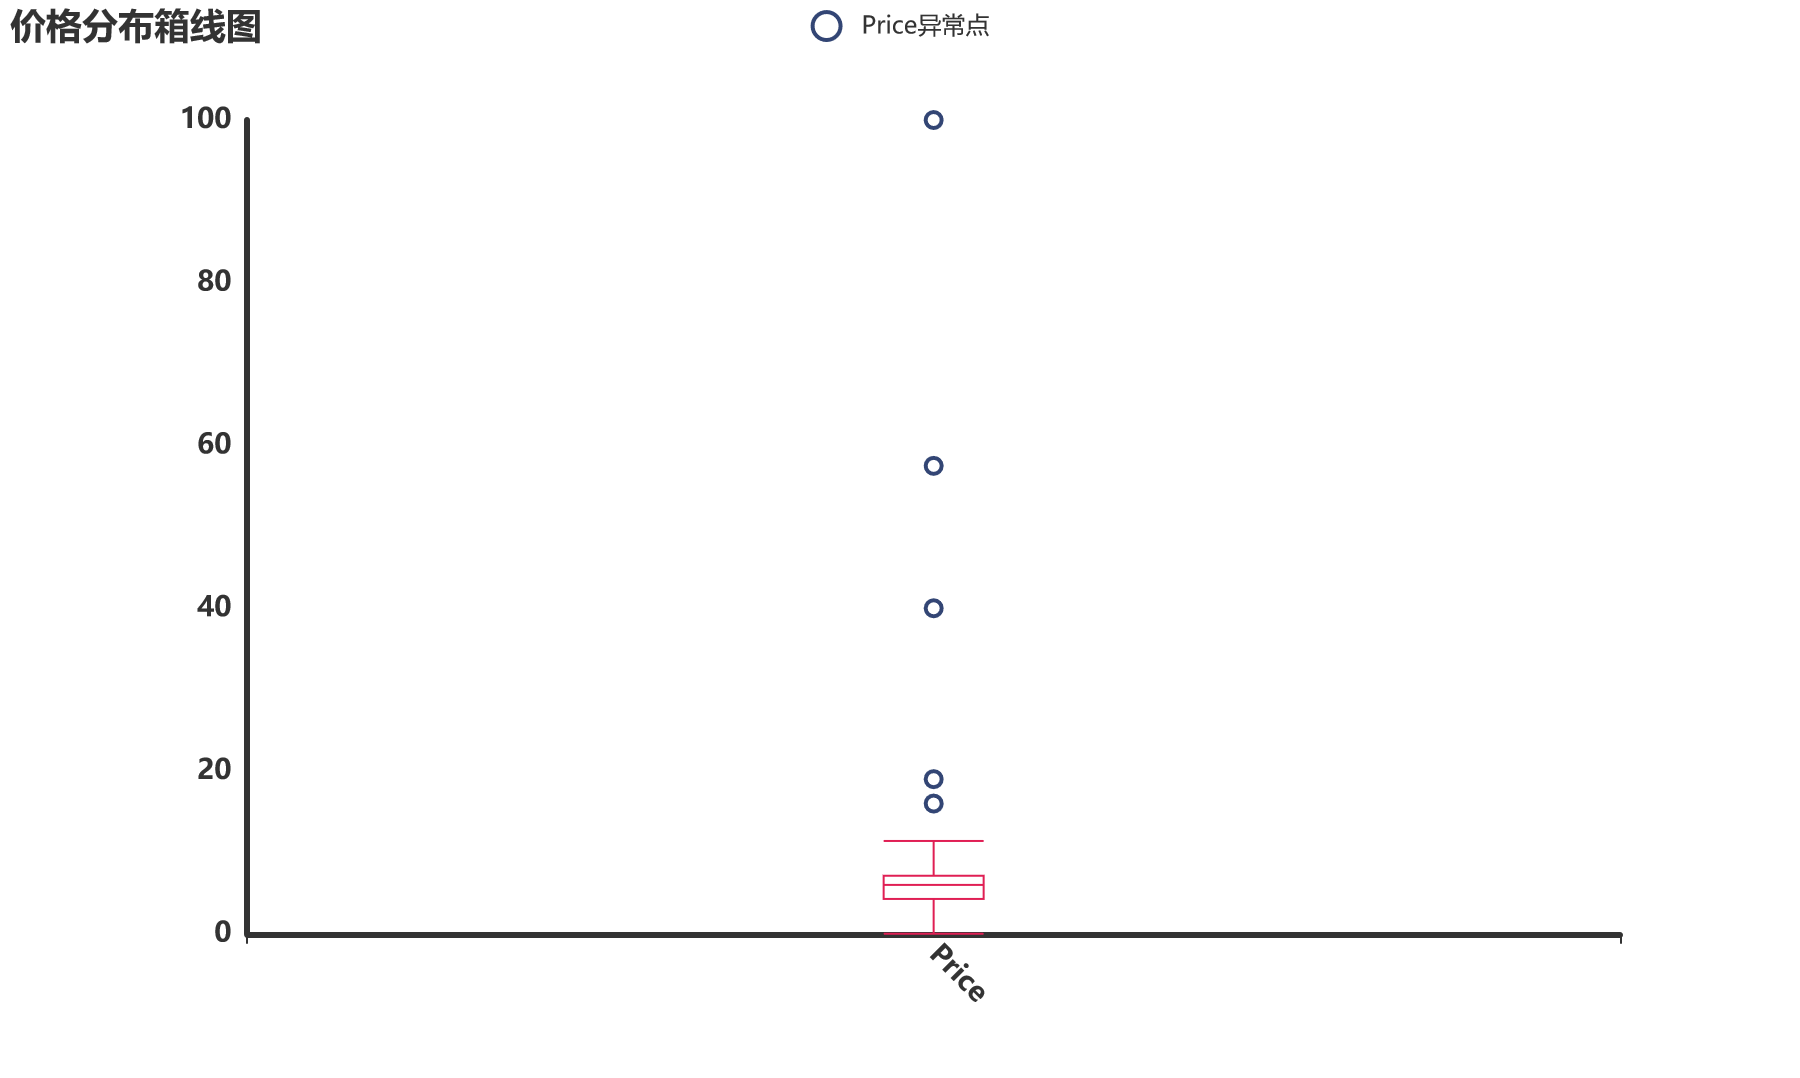
\includegraphics[width=0.9\textwidth]{figures/preprocess/preprocess1.png}
  \caption{销售单价异常值检测}
  \label{fig:preprocess1}
\end{figure}


在对农作物种植策略进行优化之前,数据的清洗和预处理是至关重要的步骤。
数据预处理的质量直接影响模型分析的结果和优化策略的准确性。
本文提供的多个Excel文件(附件1、附件2以及结果模板)包含了乡村的耕地信息、2023年农作物种植和相关统计数据等基础数据。
这些数据在实际应用中可能存在格式不规范、异常值和缺失数据等问题,因此我们需要通过严格的预处理步骤,确保数据的质量和一致性。


\subsection{数据清洗与格式规范化}

在初步分析Excel文件时,我们发现部分单元格中的文本和数字存在多余的空格,尤其是在一些农作物名称、地块类型以及销售单价等字段中,这些空格可能是在数据录入过程中无意输入的。
尽管这些空格在视觉上可能不会明显影响数据的展示,但它们会对后续的数据处理和分析带来问题。
例如,多余的空格可能导致同一作物被视为不同的条目,进而影响模型对数据的准确性。
因此,清理这些空格是数据预处理中的首要任务。


我们采用了自动化数据清洗的方式,通过编写 Python 脚本,使用\texttt{strip()}函数去除所有文本字段中的多余空格。
同时,针对数值型数据,我们检查了是否存在与单位不一致的情况(如数字后跟随空格或特殊字符),并对其进行了统一处理。
通过这些步骤,所有农作物的名称、地块类型、销售价格等字段得到了统一的格式,从而避免了因数据格式不一致导致的分析错误。


\subsection{异常值检测与处理}

在数据预处理中,异常值的检测是另一个重要环节。
通过对附件2中2023年乡村农作物销售单价数据的分析,我们发现了几个异常值,这些异常值表现为某些作物的单价远高于其他作物的平均水平。
如图\ref{fig:preprocess1}所示,羊肚菌、榆黄菇、荞麦、香菇和白灵菇的单价明显高于其他农作物。
这些异常值的出现可能是数据输入错误,也可能是由于这些作物本身的市场价值较高而导致的价格差异。


为了确定这些异常值是否需要被处理或保留,我们进行了进一步的分析。
首先,我们通过查询市场价格数据,发现这些农作物确实属于高价值的经济作物。
例如,羊肚菌作为一种珍贵的食用菌,其市场售价远高于一般农作物。
同样,榆黄菇、荞麦、香菇和白灵菇等作物在市场上具有较高的需求和价格。
这意味着这些高单价并非数据输入错误,而是反映了市场的真实情况。
因此,我们决定保留这些异常值,并将它们纳入后续的分析和建模中。
保留这些高价值作物能够更好地反映乡村的种植策略,并在经济效益上体现出这些作物的重要性。


\subsection{数据完整性检查}

在对Excel数据进行检查后,我们发现所有字段均无缺失数据。
这表明数据的录入和存储过程较为规范,不需要对缺失数据进行额外处理。
因此,我们可以直接对这些完整的数据进行后续的分析和建模。


虽然没有缺失数据,但我们依然对数据的合理性进行了验证,确保每个字段的数值符合实际情况。
例如,地块面积、作物产量和销售量等数据均符合乡村的实际种植情况。
经过这一数据完整性检查后,我们确认数据质量符合预期,可以直接进入下一步的数据处理和模型分析。


\subsection{数据转换与衍生变量创建}

为了更好地分析乡村的农作物种植策略,并为后续模型构建提供有效的数据支持,我们对原始数据进行了适当的转换,并创建了若干个衍生变量。
这些衍生变量能够帮助我们更深入地分析不同作物的种植效益、种植面积分配、作物轮作规律以及耕地类型对作物种植的影响。

\subsubsection{地块种植面积分配}

根据每个地块的种植面积和作物的种植面积分配情况,我们需要对各地块上不同作物的总种植面积进行计算。
对于每个地块 $i$,我们定义了总种植面积 $A_{ijk}$,它包括非大棚地块和大棚地块的种植面积。
总面积的计算公式如下:

\[
  A_{ijk} = \sum_s A_{ijks}
\]

其中,$A_{ijks}$ 表示在 $k$ 年 $s$ 季度第 $j$ 种作物的种植面积。


\subsubsection{地块类型与作物可种植集合}

不同类型的地块适合种植不同种类的作物,因此我们为每个地块 $i$ 定义了其地块类型 $t_i$,如平旱地、梯田、山坡地、智能大棚、普通大棚、水浇地等。
基于地块类型 $t_i$,我们进一步定义了地块在每一季节 $s$ 可种植的作物集合 $\hat{T}_{is}$。


例如,对于水浇地,$\hat{T}_{is}$ 可能包括 $Grains_B$(水稻)和 $Vege_A$(蔬菜);而对于普通大棚,$\hat{T}_{is}$ 可能包括 $Vege_A$ 和 $Mush$(食用菌)。
通过这一衍生变量,我们可以确保模型在作物种植时遵循地块适宜种植的原则,避免种植不适宜的作物导致产量下降或损失。


\subsubsection{作物分类与集合定义}

为了便于分析和模型优化,我们对不同作物进行了分类,并定义了若干个作物集合:

\begin{itemize}
  \item $\text{Beans}$:豆类作物的集合。
        根据题目要求,豆类作物需要在三年内至少在每个地块上种植一次,这一约束条件通过 $\text{Beans}$ 集合来实施。

  \item $\text{Grains}_A$:A类粮食作物的集合,即除了水稻之外的粮食作物。
        该集合包括小麦、玉米等作物,适合在平旱地、梯田等露天地块种植。

  \item $\text{Grains}_B$:B类粮食作物的集合,即水稻。
        水稻通常种植在水浇地中,因此 $Grains_B$ 主要用于限制水稻的种植地块选择。

  \item $\text{Vege}_A$:A类蔬菜的集合,指除了大白菜、白萝卜和红萝卜之外的蔬菜。
        该集合用于普通大棚和水浇地的种植规划。

  \item $\text{Vege}_B$:B类蔬菜的集合,包括大白菜、白萝卜和红萝卜,这些蔬菜适合种植在普通大棚和露天耕地上。

  \item $\text{Mush}$:食用菌的集合,包括羊肚菌、榆黄菇、香菇、白灵菇等高价值食用菌作物,通常种植在大棚内。

\end{itemize}

通过这些集合定义,我们能够有效地将作物分类,便于模型在不同地块、不同季节选择最优的种植作物。


通过对原始数据的转换和多个衍生变量的创建,我们显著增强了数据的维度和可操作性。
这些衍生变量不仅能够帮助我们更精确地进行作物种植效益分析,还为后续的模型优化提供了重要的参考依据。
在接下来的模型分析和求解中,我们将充分利用这些衍生变量,确保种植策略能够最大化乡村的农业收益,并实现可持续发展的目标。


\subsubsection{各地块作物种植面积的可视化分析}

为了更好地理解不同地块的资源利用情况,我们首先对每个地块的作物种植面积进行了可视化分析。
通过图\ref{fig:preprocess1}的分析可以看出,不同类型的地块在种植面积分布上存在显著差异。


\begin{figure}[H]
  \centering
  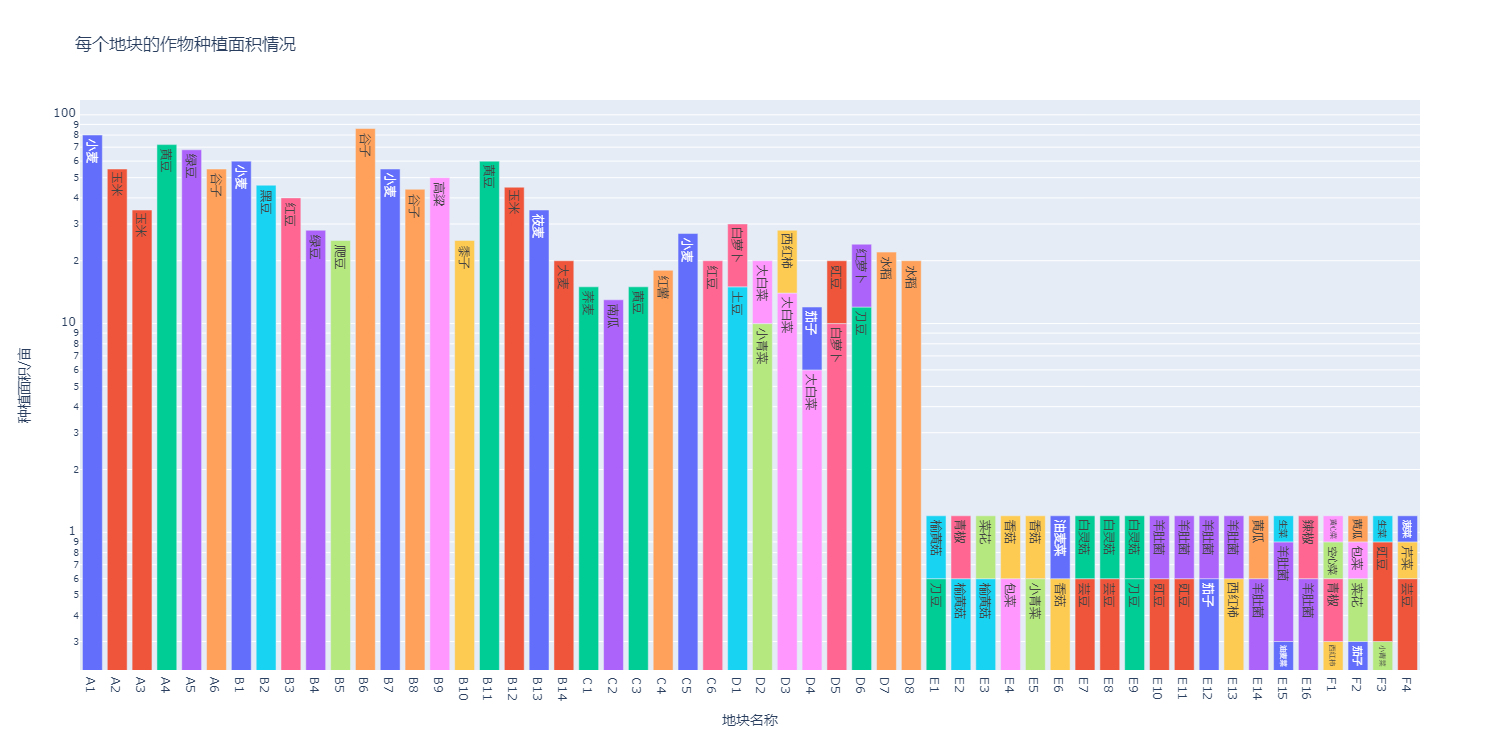
\includegraphics[width=0.8\textwidth]{figures/preprocess/每个地块的作物种植面积.png}
  \caption{每个地块的作物种植面积}
  \label{fig:preprocess1}
\end{figure}

\subsubsection{作物产量与利润分析}

\begin{figure}[H]
  \centering
  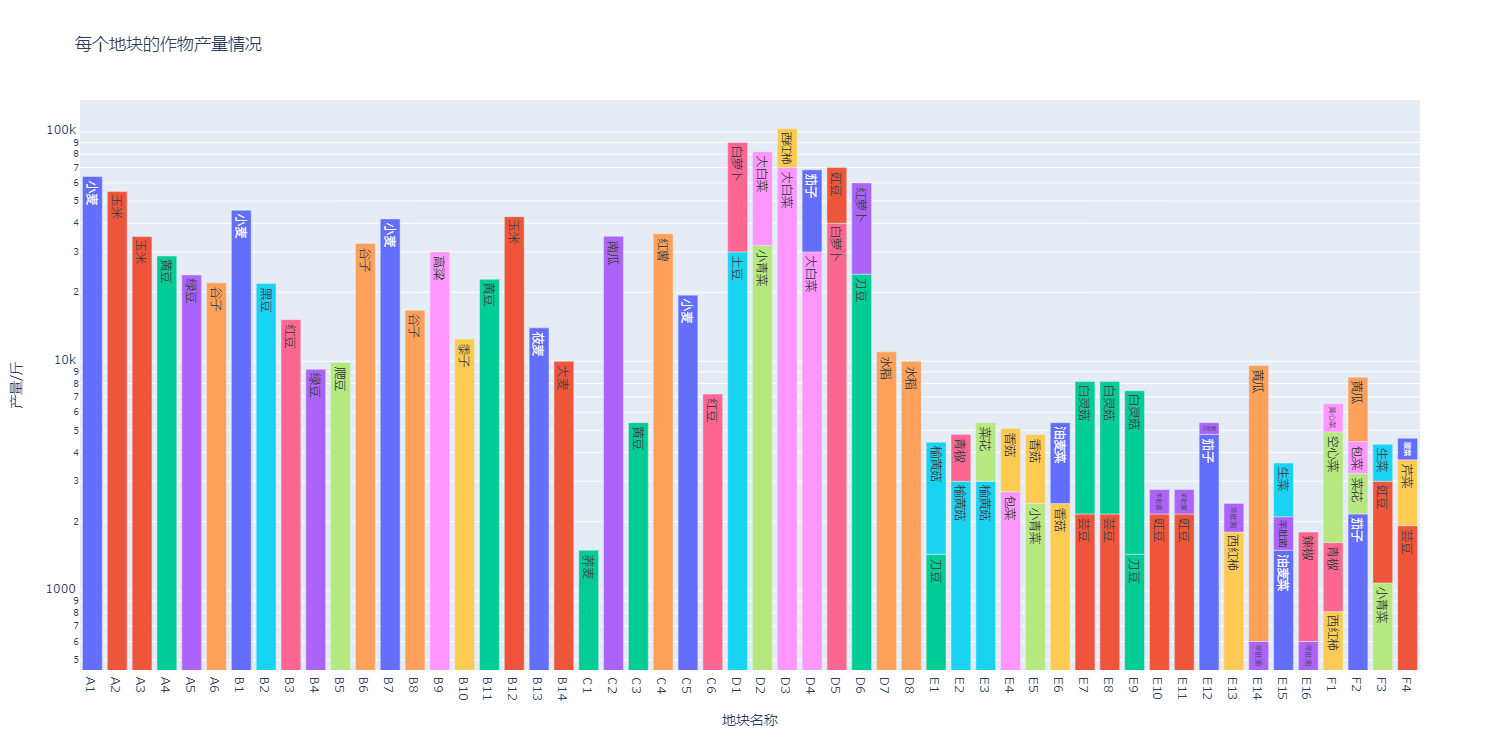
\includegraphics[width=0.8\textwidth]{figures/preprocess/每个地块的作物产量.png}
  \caption{每个地块的作物产量}
  \label{fig:preprocess2}
\end{figure}

\begin{figure}[H]
  \centering
  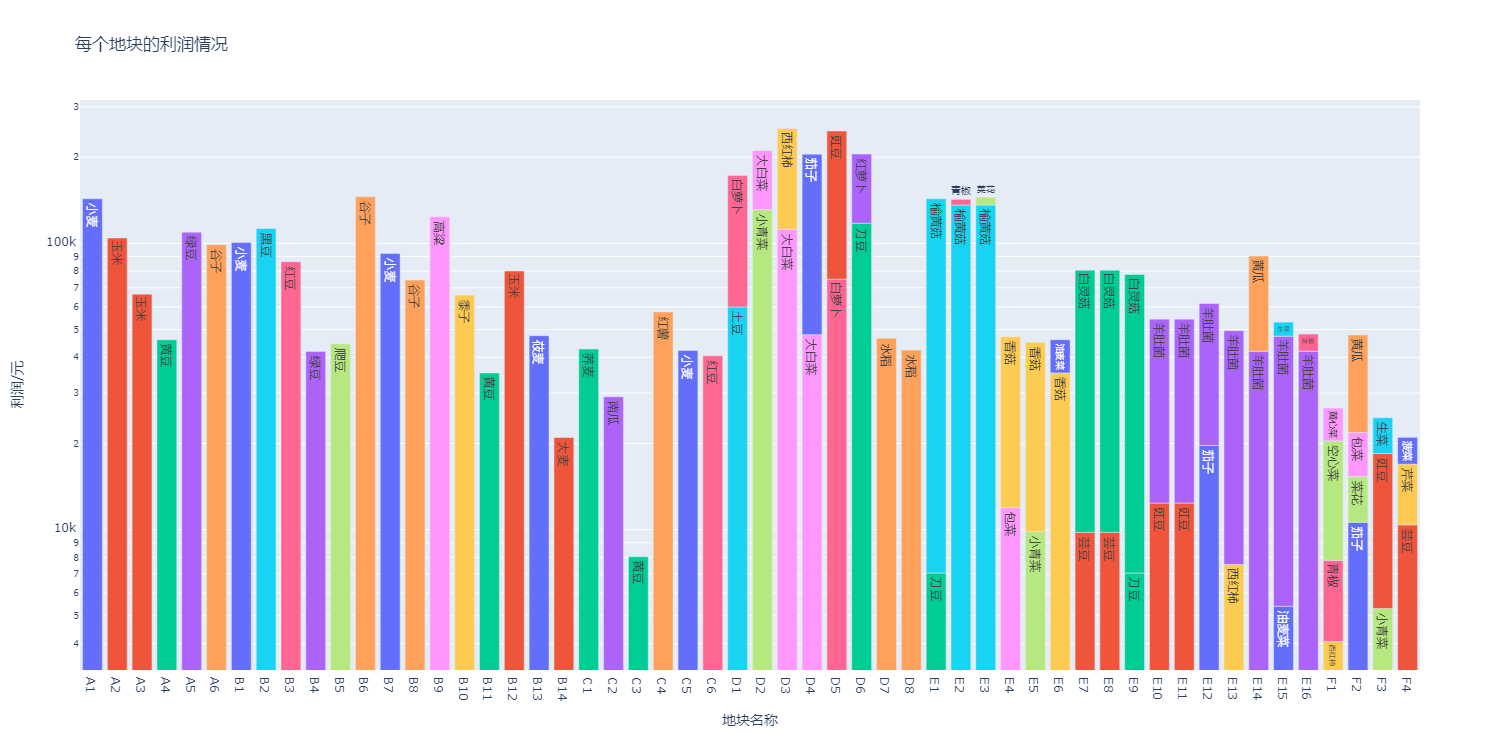
\includegraphics[width=0.8\textwidth]{figures/preprocess/每个地块的利润.png}
  \caption{每个地块的利润}
  \label{fig:preprocess3}
\end{figure}

图\ref{fig:preprocess2}展示了每个地块的作物总产量。
图\ref{fig:preprocess3}展示了每个地块的总利润。
通过该图表,我们可以更直观地了解不同地块的经济效益。
结果表明,尽管大棚的单位面积成本较高,但其利润表现却并不低于大多数露天耕地,尤其是在高价值作物的种植上。
因此,在未来的种植策略中,调整大棚作物的种植面积或提高露天作物的产量效益会一定程度上影响整体收益。


\subsubsection{作物在不同地块下的收入表现}

为了进一步分析同一作物在不同地块类型下的表现,我们对各个地块下的作物总收入进行了统计,图\ref{fig:preprocess4}展示了同一作物在不同地块下的总收入情况。
可以发现,羊肚菌和香菇等高价值经济作物在大棚中的表现显著优于露天耕地,这进一步证明了大棚对于这些作物的经济效益的重要性。


\begin{figure}[H]
  \centering
  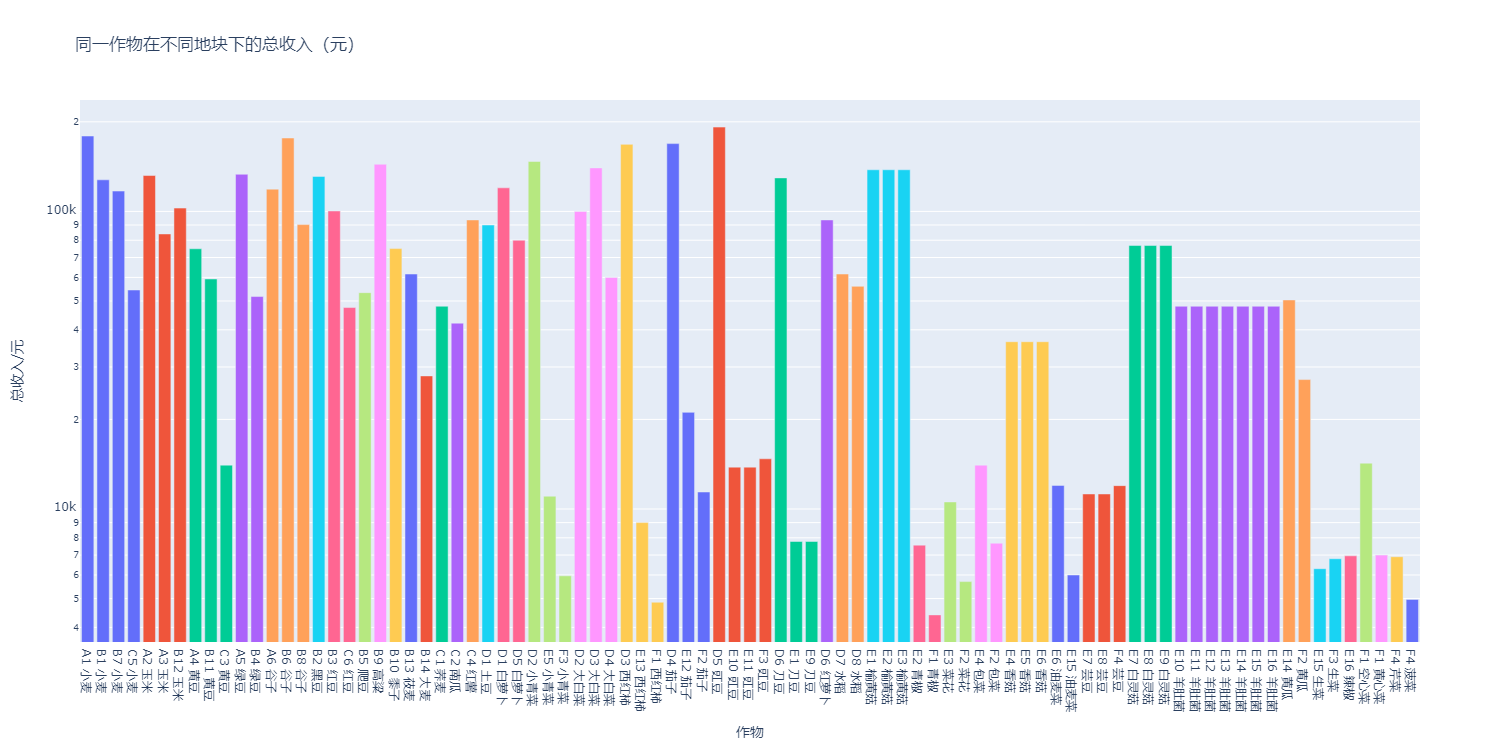
\includegraphics[width=0.8\textwidth]{figures/preprocess/同一作物在不同地块下的总收入.png}
  \caption{同一作物在不同地块下的总收入}
  \label{fig:preprocess4}
\end{figure}

\subsubsection{不同地块类型下的作物价格差异分析}

\begin{figure}[H]
  \centering
  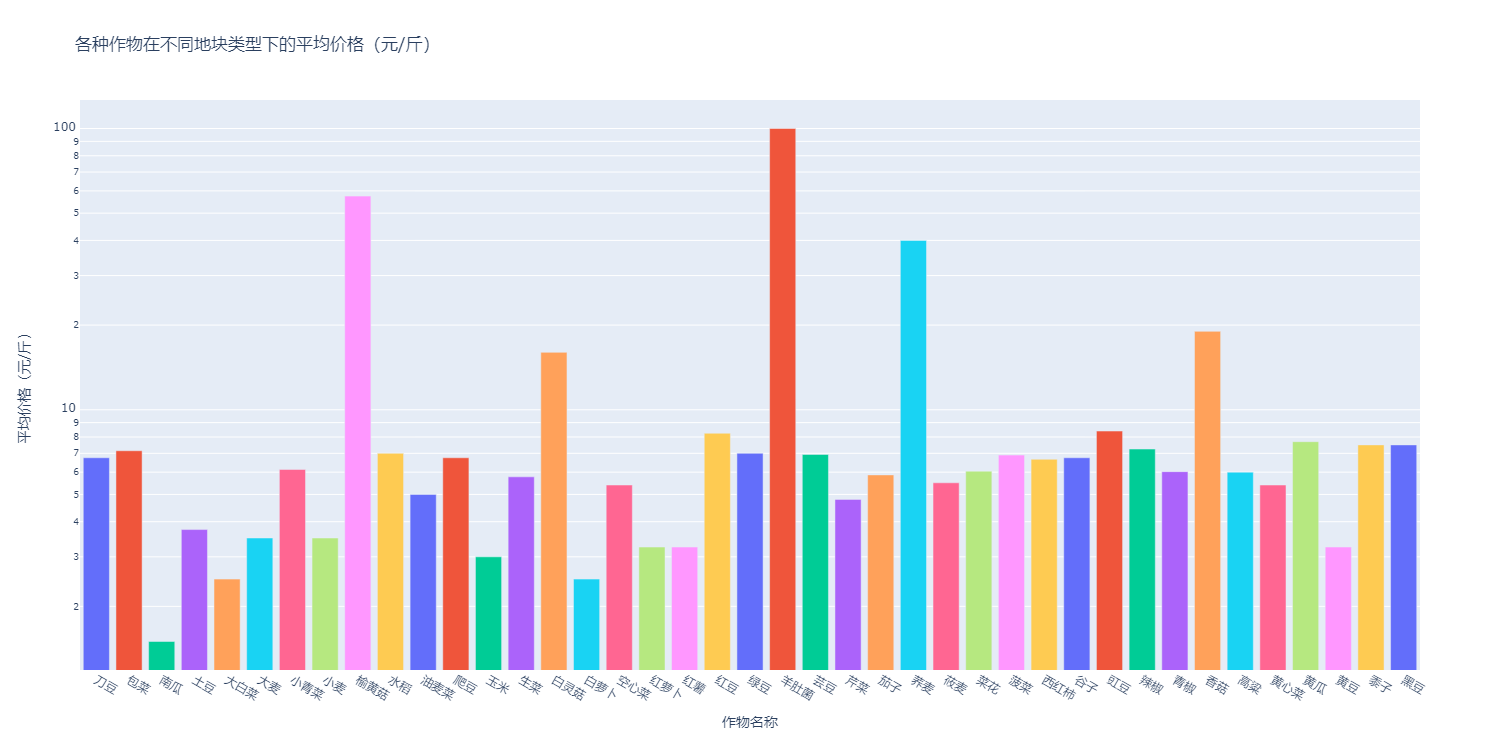
\includegraphics[width=0.8\textwidth]{figures/preprocess/各种作物在不同地块类型下的平均价格.png}
  \caption{各种作物在不同地块类型下的平均价格}
  \label{fig:preprocess5}
\end{figure}

图\ref{fig:preprocess5}展示了各种作物在不同地块类型下的平均销售价格。
通过这一分析,我们能够识别出不同地块类型对作物销售价格的影响。
大棚作物的平均价格普遍高于露天作物,尤其是对于高价值的经济作物,这一现象尤为显著。





%%%%%%%%%%%%%%%%%%%%%%%%%%%%%%%%%%%%%%%%%%%%%%%%%%%%%%%%%%%%%%%%%%

\section{问题一的模型建立与求解}

\subsection{思路分析}

问题一要求为乡村制定2024至2030年的最优农作物种植策略。
该问题涉及到两种不同的情境:

\begin{enumerate}
  \item
        当作物的总产量超过预期销售量时,超出部分会滞销并造成浪费;
  \item
        超出部分按2023年销售价格的50\%降价出售。
        在这两种情境下,我们的目标是通过合理分配有限的耕地资源,最大化乡村的经济效益。

\end{enumerate}


这类问题可以归类为典型的资源分配优化问题,具体表现为如何在多种作物之间合理分配有限的土地资源,以满足市场需求、最大化种植收益,并避免资源浪费。
为了实现这一目标,我们构建了数学优化模型,通过设置目标函数来衡量经济效益,同时引入各种约束条件(如作物轮作、地块面积限制、最低种植面积要求等)以确保分配方案的合理性。


由于问题中的目标函数存在非线性项,使得直接求解变得复杂。
为了简化模型的求解过程,我们引入了辅助变量 $z_{ijk}$,用于替代目标函数中非线性部分的表示,并将其线性化处理。
通过这样的引入,我们能够将原始非线性模型转化为线性规划问题,使得模型能够通过现有的线性规划求解方法(如Pulp库)进行求解。


我们将基于这两种情境分别定义目标函数,并设置相应的约束条件,确保所设计的种植方案符合实际操作需求,尤其是考虑到作物的轮作要求、地块种植面积限制等。
此外,还需要保证每种作物在单个地块上的最小种植面积,从而避免土地资源分配过于分散带来的管理成本过高问题。


\subsection{决策变量}

在本模型中,决策变量主要涉及农作物的种植面积分配。
为合理分配大棚地块和非大棚地块的种植面积,我们定义以下决策变量:
\begin{itemize}
  \item $A_{ijks}$:在 $k$ 年 $s$ 季度的第 $i$ 块土地种植 $j$ 种作物的面积。
\end{itemize}

为了将线性化函数中的非线性部分和约束条件的逻辑部分转化为标准线性规划形式,我们引入如下辅助变量
\begin{itemize}
  \item $z_{ijk}$:表示第 $k$ 年第 $j$ 种作物的超出预期销售量的部分,即:
        \[
          z_{ijk} = \max(0, Y_{jk} \cdot A_{ijk} - S_{jk})
        \]
        其中,$Y_{jk}$ 是单位面积的产量,$A_{ijk}$ 是总种植面积,$S_{jk}$ 是期望销售量。


\end{itemize}

\subsection{目标函数}

模型的目标是最大化经济收益。
在问题一中,我们针对两种不同的情境,分别定义了两个目标函数。


\subsubsection{情况一:作物超出部分滞销}

在情况一中,如果某种作物的总产量超过了预期销售量,超出部分将滞销并造成浪费。
在这种情况下,目标函数旨在最大化可销售的产量收益,同时扣除种植成本。
具体公式如下:
\[
  L_1 = \sum_{ijk} \left( \min(S_{jk}, Y_{jk} \cdot A_{ijk}) \cdot P_{jk} - C_{jk} \cdot A_{ijk} \right)
\]
其中:
\begin{itemize}
  \item $S_{jk}$:第 $k$ 年第 $j$ 种作物的期望销量;
  \item $Y_{jk}$:第 $k$ 年第 $j$ 种作物的单位面积产量;
  \item $P_{jk}$:第 $k$ 年第 $j$ 种作物的售价;
  \item $C_{jk}$:第 $k$ 年第 $j$ 种作物的单位面积成本;
  \item $A_{ijk}$:第 $i$ 地块上,第 $j$ 种作物的总种植面积;
\end{itemize}

\subsubsection{情况二:超出部分按50\%降价出售}

在情况二中,超出期望销售量的部分将按2023年销售价格的50\%降价出售。
对于这一情况,目标函数需要考虑降价出售部分的收益,具体公式如下:
\[
  L_2 = \sum_{ijk} \left( Y_{jk} \cdot A_{ijk} \cdot P_{jk} - C_{jk} \cdot A_{ijk} - 0.5 \cdot z_{ijk} \cdot P_{jk} \right)
\]
其中:
\begin{itemize}
  \item $Y_{jk} \cdot A_{ijk}$:总产量;
  \item $C_{jk} \cdot A_{ijk}$:种植成本;
  \item $z_{ijk}$:超出期望销售量的部分;
  \item $0.5 \cdot z_{ijk} \cdot P_{jk}$:超出部分按50\%价格降价出售的收益。

\end{itemize}

通过引入辅助变量 $z_{ijk}$,我们将运算转化为线性形式,使得目标函数可以更容易地求解。


\subsection{约束条件}

为了确保模型的合理性和可操作性,我们引入了若干约束条件,包括地块面积限制、轮作规则、最小种植面积要求等。

\subsubsection{逻辑约束}

为了确保每个地块的种植面积合理分配,我们为决策变量 $A_{ijks}$ 设置上界约束:
\[
  B_{ijks} \cdot M \geq A_{ijks}, \quad M = 10000
\]
其中,$M$ 是一个大值常量(如10000),用于确保种植面积 $A_{ijks}$ 不超过允许范围。


\subsubsection{地块总面积约束}

每种作物合起来的种植面积不超过相应地块的总面积,具体公式为:
\[
  \sum_j A_{ijks} \leq A_i^* \quad \forall i,k \text{ and } j \in \hat{T}_{is}
\]
其中,$A_i^*$ 是第 $i$ 地块的总面积,$\hat{T}_{is}$ 是该地块在第 $s$ 季节可种植的作物集合。


\subsubsection{轮作规则}

轮作规则的引入主要是为了避免作物在同一地块连续种植带来的重茬问题,重茬种植可能导致土壤肥力下降、病虫害增加,从而影响作物的产量和质量。
为了应对这一问题,我们在模型中设置了如下轮作约束条件:

\begin{itemize}
  \item 对于不具备第二季种植条件的土地(如平旱地、梯田、山坡地),每年只能种植一季作物,因此需保证同一种作物不能在连续的两个年度种植在同一块地上,约束条件为:
        \[
          B_{ijks} + B_{ij(k+1)s} \leq 1, \quad t_i \in \{\text{平旱地}, \text{梯田}, \text{山坡地}\}, \forall j, k, s
        \]

  \item 对于具备多季种植条件的土地(如水浇地、普通大棚等),在同一年内也不能在连续的两个季节种植同一种作物,约束条件为:
        \[
          B_{ijks} + B_{ijk(s+1)} \leq 1, \quad t_i \in \{\text{水浇地}, \text{普通大棚}, \text{智慧大棚}\}, T_{i2} \neq \emptyset
        \]
\end{itemize}

\subsubsection{豆类作物轮作约束}

根据题目要求,每个地块三年内至少需要种植一次豆类作物。
豆类作物由于具有根瘤菌固氮的功能,可以为土壤提供额外的氮肥,有助于改善后续作物的生长环境。
因此,豆类作物的轮作不仅能够提高土壤肥力,还可以减少化肥的使用,降低农业生产成本。


为了满足这一要求,我们设置以下约束条件:
\begin{itemize}
  \item 首先确保每块地三年内至少种植一次豆类作物:
        \[
          \sum_{k=t_0}^{t_0+2} \sum_s B_{ijks} \geq 1, \quad t_0 \in \{2024, 2025, \dots, 2028\}, \quad j \in \text{Beans}, \forall i
        \]
        该约束条件确保在三年内(即从 $t_0$ 到 $t_0 + 2$ 年)至少有一季种植豆类作物,$t_0$ 表示起始年份,而 $j \in \text{Beans}$ 则限定了种植的作物必须为豆类。
        这样可以确保每块地的土壤在三年内都能得到豆类作物的修复作用,从而长期保持土地的健康和高效产出。


  \item 其次,确保每次种植的豆类作物覆盖整块土地,而不是只种植部分区域。
        为此,我们引入以下面积约束:
        \[
          A_{i}^* B_{ijks} = A_{ijks}, \quad j \in \text{Beans}, \forall i,k,s
        \]
        该约束条件确保当 $B_{ijks} = 1$(即种植豆类作物时),种植面积 $A_{ijks}$ 必须等于该地块的总面积 $A_{i}^*$,从而确保豆类作物轮作的效果覆盖整块土地,发挥其最大化的土壤改良效果。

\end{itemize}

\subsubsection{最小种植面积限制}

在实际种植中,为了保证种植效益和田间管理的便捷性,避免某些作物的种植面积过小导致管理成本过高的问题,我们还需要为每种作物的种植面积设定最低面积限制。


具体来说,我们引入了如下约束条件,确保每种作物在每块地上的种植面积不低于总地块面积的一定比例:
\[
  A_{ijks} \geq \epsilon \cdot A_{i}^*, \quad \text{if } B_{ijks} = 1, \quad \forall i,k,j,s
\]
其中,$\epsilon$ 是最小面积比例系数,根据2023年的数据分析,取值为 $\epsilon = 0.3$。
这意味着每次种植的面积至少应为地块总面积的30\%,以确保田间管理的便捷性并避免种植面积过小造成的资源浪费和效率低下。


该最小面积约束对于实际生产具有较大意义,尤其是在土地资源有限的条件下,保证作物种植的规模效益是优化种植方案的重要考虑因素。
通过该约束条件,模型可以排除那些面积过小、管理成本较高的种植方案,从而提高整体的种植效益。


\subsubsection{地块种植限制}

不同地块具有不同的土壤条件、气候条件以及水资源条件,这在很大程度上决定了每块地适合种植的作物种类。
因此,为了确保种植方案的可行性和合理性,我们根据地块的类型设置了种植限制,确保每块地在不同季节种植合适的作物。

地块种植限制的具体如下:
\begin{itemize}
  \item 平旱地、梯田、山坡地:
        \[
          \hat{T}_{i1} = \text{Grains}_A, \quad \hat{T}_{i2} = \emptyset, \quad t_i \in \{\text{平旱地}, \text{梯田}, \text{山坡地}\}
        \]
        其中,$\hat{T}_{i1}$ 表示第一季度可以种植的作物类型集合,$\text{Grains}_A$ 包含小麦、玉米等适合此类地块的粮食作物。
        而 $\hat{T}_{i2} = \emptyset$ 表示这些地块每年只能种植一季作物,第二季不适合继续种植。


  \item 水浇地:
        \[
          \hat{T}_{i1} = \text{Grains}_B \quad \text{或} \quad \hat{T}_{i1} = \text{Vege}_A, \quad \hat{T}_{i2} = \text{Vege}_B, \quad t_i \in \{\text{水浇地}\}
        \]
        在第一季度,水浇地可以种植水稻($\text{Grains}_B$)或蔬菜($\text{Vege}_A$)。
        而在第二季度,水浇地适合种植根茎类蔬菜($\text{Vege}_B$),如大白菜、白萝卜等。


  \item 普通大棚:
        \[
          \hat{T}_{i1} = \text{Vege}_A, \quad \hat{T}_{i2} = \text{Mush}, \quad t_i \in \{\text{普通大棚}\}
        \]
        通常,第一季种植蔬菜($\text{Vege}_A$),第二季则可以种植食用菌($\text{Mush}$)



  \item 智慧大棚:
        \[
          \hat{T}_{i1} = \hat{T}_{i2} = \text{Vege}_A, \quad t_i \in \{\text{智慧大棚}\}
        \]
        第一季和第二季都种植($\text{Vege}_A$)。

\end{itemize}

我们可以将其表示为约束条件如下:
\[
  \hat{T}_{is} =
  \begin{cases}
    \begin{aligned}
       & \hat{T}_{i1} = \text{Grains}_A, \quad \hat{T}_{i2} = \emptyset, \quad & \text{if } t_i \in \{\text{平旱地}, \text{梯田}, \text{山坡地}\} \\
    \end{aligned}                                \\
    \begin{aligned}
       & \hat{T}_{i1} = \text{Grains}_B \quad \text{或} \quad \hat{T}_{i1} = \text{Vege}_A, \quad \hat{T}_{i2} = \text{Vege}_B, \quad & \text{if } t_i \in \{\text{水浇地}\}
    \end{aligned} \\
    \begin{aligned}
       & \hat{T}_{i1} = \text{Vege}_A, \quad \hat{T}_{i2} = \text{Mush}, \quad & \text{if } t_i \in \{\text{普通大棚}\}
    \end{aligned}                                                      \\
    \begin{aligned}
       & \hat{T}_{i1} = \hat{T}_{i2} = \text{Vege}_A, \quad & \text{if } t_i \in \{\text{智慧大棚}\}
    \end{aligned}
  \end{cases}
\]

\subsubsection{辅助变量约束条件}

在目标函数的设计过程中,我们引入了辅助变量 $z_{ijk}$,用于表示作物的实际产量与预期销售量之间的差值。
这些辅助变量的引入有助于将目标函数中的非线性部分线性化处理,从而便于模型的求解。


为了确保辅助变量的合理性,我们需要对 $z_{ijk}$ 施加一定的约束条件。
具体来说,辅助变量 $z_{ijk}$ 的值应该是实际产量 $Y_{jk} \cdot A_{ijk}$ 减去期望销售量 $S_{jk}$,但不能为负数。
因此,辅助变量的约束条件可以表示为:

\begin{itemize}
  \item 非负性约束:辅助变量 $z_{ijk}$ 必须为非负值,确保其仅表示超出部分的产量。
        具体约束为:
        \[
          z_{ijk} \geq 0, \quad \forall i, j, k
        \]
        该约束确保辅助变量不会出现负值,即当实际产量未超过预期销售量时,$z_{ijk} = 0$,表示没有超出部分。


  \item 最优性约束:辅助变量 $z_{ijk}$ 必须大于等于实际产量减去期望销售量的差值。
        具体约束为:
        \[
          z_{ijk} \geq Y_{jk} \cdot A_{ijk} - S_{jk}, \quad \forall i, j, k
        \]
        这一约束确保 $z_{ijk}$ 精确表示超出部分的产量,即当 $Y_{jk} \cdot A_{ijk} > S_{jk}$ 时,$z_{ijk}$ 等于 $Y_{jk} \cdot A_{ijk} - S_{jk}$,否则 $z_{ijk} = 0$。

\end{itemize}


\subsubsection{模型的完整性与可操作性}

通过以上详细的决策变量、目标函数、约束条件和辅助变量的设置,我们已经建立了一个完整且具备可操作性的优化模型。
这个模型能够充分考虑到实际种植中的各种限制条件,如土地类型的限制、作物的轮作需求、种植面积的分配等,并通过线性化处理,使得模型能够在现有的线性规划求解方法中高效求解。

该建模过程将复杂的多约束条件和多目标问题转化为了线性规划问题,并通过引入辅助变量解决非线性问题的求解难题。
最终的目标是为乡村提供一个科学合理的种植方案,在应对不确定性和市场波动的同时,确保农作物产量和经济收益的最大化。



\subsection{模型求解思路}

在确定了模型的决策变量、目标函数和约束条件之后,我们可以通过线性规划(Linear Programming, LP)技术对问题一的种植面积分配问题进行求解。
线性规划是一种适用于资源分配问题的优化方法,尤其在处理具有线性目标函数和线性约束条件的问题时,效果尤为显著。
基于本问题的实际场景,种植面积的分配问题可以通过标准的线性规划求解算法,如单纯形法(Simplex Method)或内点法(Interior Point Method)来求得最优解。


\subsubsection{线性规划的应用}

在情况一和情况二下,目标函数分别为 $L_1$ 和 $L_2$。
这两个目标函数都是关于种植面积 $A_{ijk}$ 的线性函数,尽管形式略有不同,但它们都可以归结为标准的线性优化问题。
我们的目标是通过优化地块上各类作物的种植面积 $A_{ijk}$,使得在约束条件的限制下,最大化乡村的总收益。


对于情况一,目标函数 $L_1$ 可表示为:

\[
  L_1 = \sum_{ijk} \left( \min \left( S_{jk}, Y_{jk} \cdot A_{ijk} \right) \cdot P_{jk} - C_{jk} \cdot A_{ijk} \right)
\]

其中,$A_{ijk}$ 是第 $i$ 地块上第 $j$ 种作物在第 $k$ 年的总种植面积,$Y_{jk}$ 是单位面积的产量,$S_{jk}$ 是期望销售量,$P_{jk}$ 是作物的单位售价,$C_{jk}$ 是单位种植成本。
在情况一中,若作物总产量 $Y_{jk} \cdot A_{ijk}$ 超出期望销售量 $S_{jk}$,超出的部分不产生收益,导致滞销。


对于情况二,目标函数 $L_2$ 可表示为:

\[
  L_2 = \sum_{ijk} \left( Y_{jk} \cdot A_{ijk} \cdot P_{jk} - C_{jk} \cdot A_{ijk} - 0.5 \cdot z_{ijk} \cdot P_{jk} \right)
\]

这里,$z_{ijk}$ 是辅助变量,表示作物超出预期销售量的部分,$z_{ijk} = \max(0, Y_{jk} \cdot A_{ijk} - S_{jk})$。
在情况二中,超出的部分按50\%的降价出售,导致收益部分下降。


为将这些目标函数表示为标准的线性规划形式,我们引入了辅助变量 $z_{ijk}$,以简化 $L_2$ 中非线性部分 $\max(0, Y_{jk} \cdot A_{ijk} - S_{jk})$ 的处理。
线性规划的标准形式为:

\[
  \max \ L_1 \quad \text{或} \quad \max \ L_2
\]
\[
  \text{subject to} \ \text{constraints on } A_{ijk}, z_{ijk}
\]

这些约束条件包括地块总面积限制、作物轮作要求、豆类作物轮作、最小种植面积限制等,都是线性约束,因此我们可以通过线性规划求解算法来寻找最优解。


\subsubsection{模型求解过程}

在模型求解过程中,我们使用了 Pulp 库中的 \texttt{prob.solve()} 函数。
Pulp 是 Python 的线性规划求解库,它可以将目标函数、约束条件以数学模型的形式定义,并通过求解器来找到最优解。

\paragraph{求解器选择与配置}

Pulp 提供了多种求解器选项,包括 GLPK、CBC 等。
在我们的模型中,默认使用的是 CBC(Coin-or branch and cut)求解器。
CBC 是一种高效的线性规划和混合整数规划求解器,特别适合处理大规模的线性优化问题。
由于问题一中的决策变量 $A_{ijk}$ 是连续变量,并且模型是线性规划问题,CBC 求解器能够在较短的时间内找到最优解。


求解器会根据定义的目标函数和约束条件,自动将问题转换为线性规划问题,并通过迭代优化的方式找到每个地块上最优的作物种植面积分配。


\subsubsection{线性规划求解原理}

线性规划通过优化算法在解空间中寻找目标函数的最优值,常用算法包括单纯形法和内点法。


\textbf{单纯形法}通过在解空间顶点之间移动,逐步逼近最优解。
决策变量 $A_{ijk}$ 构成的解空间由约束条件定义,如地块总面积限制和轮作规则。
算法通过迭代优化目标函数,找到最大化总收益的种植方案。


\textbf{内点法}在解空间内部沿目标函数梯度优化,适合大规模问题。
它通过内部搜索找到最优种植方案,不局限于顶点,能够在更大的解空间内找到最优解。


\textbf{边界解}出现在约束条件饱和时,例如种植面积达到上限。
\textbf{内点解}表示种植面积未达到最大限制,通常因市场需求低或种植成本高。


\paragraph{终止条件与判定}
线性规划通过迭代优化,依据目标函数改进值、可行性、无界性和不可行性判定终止。
退化解表示某些变量为零,多重最优解则存在多个相同收益的方案。


\subsubsection{思路总结}

在整个模型的求解过程中,单纯形法和内点法都通过不断迭代来逐步逼近最优解。
在每次迭代中,算法会根据当前的解,更新决策变量 $A_{ijk}$ 和辅助变量 $z_{ijk}$ 和 $B_{ijks}$的取值。
由于模型的目标是最大化总收益,因此每一次迭代的目标都是在满足所有约束条件的前提下,尽可能提高目标函数 $L_1$ 或 $L_2$ 的值。

最终的种植方案将满足以下条件:
\begin{itemize}
  \item 地块总面积限制:种植面积 $A_{ijk}$ 不超过地块的物理面积 $A_i^*$,即:
        \[
          \sum_j A_{ijks} \leq A_i^*, \quad \forall i, k, s
        \]
  \item 轮作规则:每种作物的轮作频率符合约定的轮作规则,避免了重茬种植的情况。

  \item 豆类作物的轮作要求:每个地块三年内至少种植一次豆类作物,满足土壤肥力恢复的需求。

  \item 最小种植面积限制:每种作物的种植面积满足最小面积的要求,保证田间管理的合理性。

\end{itemize}

通过这些优化步骤,模型能够为乡村提供一个最优的种植方案,不仅提高了作物的经济效益,还保证了土地资源的合理利用。


\subsection{模型求解的结果与分析}

在对模型进行求解之后,我们得到了最优的种植面积分配结果。
通过优化算法为每个地块、每种作物以及每个季度计算出了最优的种植面积,并最大化种植收益。

对于情况一,模型求解的结果将确保在作物未超出预期销售量的条件下,种植面积最大化收益,而超出部分的产量将被视为滞销。
对于情况二,超出部分的作物以50\%折扣出售,模型通过调整种植面积和分配超出产量的销售比例来优化总收益。


\subsubsection{情况一的求解结果分析}

在情况一中,农作物的总产量不能超出预期销售量。
模型通过优化种植面积,确保作物的产量刚好满足预期销售量,从而避免浪费。
通过对不同作物的产量和市场需求进行分析,模型会优先分配高收益作物的种植面积,减少低收益作物的种植。


求解结果表明,豆类作物的种植面积显著增加,原因在于其具有高市场需求和轮作要求。
此外,粮食类作物(如小麦、玉米)的种植面积分配相对稳定,蔬菜类作物则由于季节性限制,其种植面积在不同季度之间有所波动。


\subsubsection{情况二的求解结果分析}

在情况二中,模型允许超出预期销售量的部分作物以50\%的价格出售,这为优化种植策略提供了更大的灵活性。
在这一情境下,作物的种植面积分配不再仅仅受到市场需求的限制,而是可以通过适当增加某些作物的种植面积来获取更多的降价销售收益。
模型会通过平衡降价销售的潜在收益与正常市场销售的收益,来决定每种作物的最优种植面积。


求解结果表明,模型在某些高产量、高需求作物上适度增加了种植面积,尽管部分产量超出了市场需求,但通过降价出售,整体收益仍得到了提高。
例如,水稻($Grains_B$)和部分蔬菜类作物(如大白菜、白萝卜)的种植面积在情况二中相较于情况一有所增加。
特别是水稻,由于其市场需求相对稳定,即使部分产量降价出售,整体经济效益依然较高。
因此,模型倾向于在水浇地等适宜水稻种植的地块上增加水稻的种植面积。


另一方面,低收益作物(如部分豆类作物和食用菌)的种植面积在情况二中有所减少。
这是因为这些作物的市场售价较高,但其需求弹性较小,降价出售后的收益不明显。
因此,模型会优先减少这些作物的种植面积,以避免降价出售带来的收益损失。
通过这种方式,模型在作物种植面积分配上实现了不同作物的动态调整,确保整体收益在两种情境下都能够得到最大化。


\subsection{求解结果的实际应用与讨论}

模型求解的结果为乡村在2024至2030年期间的农作物种植策略提供了明确的指导。
在不同的情境下,最优种植面积的分配方式能够有效平衡市场需求、种植成本和潜在的降价风险。
然而,在实际应用中,我们还需要结合更多的现实因素来进一步优化模型结果。


\subsubsection{种植成本的动态调整与优化}

在问题一中,我们假设农作物的种植成本保持不变。
然而,随着劳动力、肥料、灌溉等成本的波动,种植成本在实际操作中会发生变化。
因此,模型可以进一步引入种植成本的动态调整机制。
例如,通过对不同年份的成本变化趋势进行预测(如使用指数平滑法或回归分析),我们可以在模型中动态调整每种作物的种植成本。

对于高成本作物,如食用菌($\text{Mush}$)和部分高价值蔬菜(如白灵菇),种植成本波动对整体收益的影响较大。
在种植成本上升时,模型可能需要减少这些作物的种植面积,转而增加低成本、高产量的粮食类作物(如小麦、玉米)的种植面积。
通过这种方式,乡村可以在面对种植成本波动时,优化种植策略以最大化收益。

\section{问题二的模型建立与求解}

\subsection{问题描述与思路分析}

在问题二中,乡村需要在2024至2030年期间制定最优的农作物种植策略,综合考虑农作物的预期销售量、亩产量、种植成本、销售价格的波动性以及潜在的种植风险。

根据题目描述,小麦和玉米的销售量未来有5\%-10\%的增长趋势,而其他农作物的销售量每年在2023年的基础上有±5\%的变化。
种植成本也会因市场条件平均每年增长5\%左右。
粮食类作物的销售价格较为稳定,而蔬菜类作物的销售价格则每年平均增长5\%,食用菌(尤其是羊肚菌)的销售价格则每年下降1\%-5\%。

考虑到各类作物的产量、成本和销售价格的年度��化。
在建模过程中,决策变量和目标函数的结构与问题一类似,但目标函数的动态性和约束条件的复杂性有所增加。


\subsection{决策变量}

与问题一相同,模型的核心决策变量是种植面积 $A_{ijk}$,它表示在第 $k$ 年第 $i$ 地块上种植第 $j$ 种作物的面积。
在问题二中,由于作物的预期销量、产量、成本和售价在不同年份有所波动,种植面积的分配需要动态调整,以适应这些变化。


\subsection{目标函数}

问题二中的目标函数与问题一类似,都是通过最大化种植收益来优化作物的种植面积分配。然而,在问题二中,作物的预期销量、产量、成本和售价都有波动,因此目标函数需要考虑这些动态变化。我们根据两种情境定义目标函数。

\subsubsection{情况一:作物超出部分滞销}

如果某种作物的总产量超过了预期销售量,超出部分将被视为滞销,因此目标函数应最大化可销售部分的收益。
目标函数表达式如下:

\[
  L_1 = \sum_{ijk} \left( \min(S_{jk} \cdot (1 + \delta_s), Y_{jk} \cdot A_{ijk}) \cdot P_{jk} - C_{jk} \cdot (1 + \delta_c) \cdot A_{ijk} \right)
\]

其中,$S_{jk}$ 是第 $k$ 年第 $j$ 种作物的预期销量,考虑年度变化因子 $\delta_s$,每年可能在5\%-10\%的范围内波动;$C_{jk}$ 是第 $k$ 年第 $j$ 种作物的单位面积种植成本,考虑年度增长因子 $\delta_c$,每年平均增长5\%。

\subsubsection{情况二:超出部分按50\%降价出售}

在这一情境中,超出预期销售量的作物将以50\%的价格降价出售。因此,目标函数需要计算超出部分的折扣收益,具体表达式如下:

\begin{align*}
  L_2 = & \sum_{ijk} \left( Y_{jk} \cdot A_{ijk} \cdot P_{jk}
  - C_{jk} \cdot (1 + \delta_c) \cdot A_{ijk} \right.           \\
        & \left. - 0.5 \cdot \max\left( 0, Y_{jk} \cdot A_{ijk}
  - S_{jk} \cdot (1 + \delta_s) \right) \cdot P_{jk} \right)
\end{align*}


在此情境下,模型允许作物的种植面积超出市场需求,超出部分将以50\%的价格出售。$0.5 \cdot \max(0, Y_{jk} \cdot A_{ijk} - S_{jk})$ 计算超出部分的折扣销售收益。

\subsection{约束条件}

问题二除了与问题一相同的约束条件外,还需要考虑农作物产量和市场价格的波动。
我们保留了问题一的基本约束条件,并在此基础上增加了关于作物销售量和价格变化的动态约束。


\subsubsection{年度销售量和价格波动约束}

由于问题二中题目明确指出了未来几年内作物销售量和售价的波动,我们需要对这些变量进行动态调整,并在约束条件中体现出年度变化的影响。
小麦和玉米的销售量预计每年增长5\%-10\%,而其他作物的销量波动在±5\%之间。
因此,针对年度销售量波动的约束条件可以表述如下:

\[
  S_{jk} = S_{j2023} \cdot (1 + \delta_s) \quad \text{where } \delta_s \in [-0.05, 0.05] \quad \text{for } j \notin \text{Grains}_A
\]

\[
  S_{jk} = S_{j2023} \cdot (1 + \delta_s) \quad \text{where } \delta_s \in [0.05, 0.10] \quad \text{for } j \in \text{Grains}_A
\]

对于其他类型的作物,年度销售量会根据2023年数据在±5\%的区间内波动,而小麦和玉米($j \in \text{Grains}_A$)的销售量则在每年增长5\%-10\%之间。这一约束条件保证了模型在每一年都能够合理调整作物的种植面积,避免因销量预期变化导致的产量过剩或不足。


此外,针对售价的波动,蔬菜类作物的售价每年平均增长5\%,而食用菌(尤其是羊肚菌)的售价则每年下降1\%-5\%。
这一情况需要在模型中通过售价的年度动态变化进行处理,具体表述为:

\[
  P_{jk} = P_{j2023} \cdot (1 + 0.05) \quad \text{for } j \in \text{Vege}_A \cup \text{Vege}_B
\]

\[
  P_{jk} = P_{j2023} \cdot (1 - \delta_p) \quad \text{where } \delta_p \in [0.01, 0.05] \quad \text{for } j \in \text{Mush}
\]

年度动态价格变化约束可以使模型确保在未来几年内不同类型作物的价格变化被合理考虑,从而在每一年都能得到最优的种植收益分配方案。


\subsubsection{种植成本的年度增长限制}

与售价变化类似,种植成本也随着年份逐渐上升,平均每年增长5\%左右。
这一变化会直接影响到种植效益,因此我们需要在模型中为种植成本增加动态约束。
具体来说,种植成本 $C_{jk}$ 在每年的变化公式如下:

\[
  C_{jk} = C_{j2023} \cdot (1 + 0.05)^{k-2023}
\]


\subsubsection{作物种植限制}

此处与问题一相同。


\subsection{模型求解思路}

在问题二中,尽管农作物的销售量、价格、种植成本和产量存在年度波动,但其核心仍然是一个线性规划问题。
与问题一相似,我们依然采用线性规划的方法来确定各个地块的种植面积分配方案 $A_{ijk}$,并在此基础上优化目标函数 $L$,以实现最大化的经济效益。
不同之处在于,问题二考虑了年度动态变量的波动,这为求解增加了不确定性。
为了处理这种不确定性,我们通过蒙特卡洛模拟对这些动态变量进行随机抽样,并将其纳入线性规划的求解框架中。


\subsubsection{模型的线性规划结构}

与问题一一样,问题二的核心是通过线性规划求解作物的最优种植面积分配方案。
线性规划的基本框架仍然不变,我们依然定义决策变量 $A_{ijk}$ 代表第 $i$ 地块在第 $k$ 年种植第 $j$ 种作物的总面积。
此外,辅助变量 $z_{ijk}$ 和 $B_{ijk}$ 也被引入,用于处理作物产量超过预期销售量时的处理方式。

由于模拟次数较多带来的时间紧迫性,我们只针对问题一中的情况一进行了研究,因此问题二模型的目标函数为:

\[
  L_1 = \sum_{ijk} \left( \min(S_{jk}, Y_{jk} \cdot A_{ijk}) \cdot P_{jk} - C_{jk} \cdot A_{ijk} \right)
\]
其中,$S_{jk}$ 表示第 $k$ 年第 $j$ 种作物的期望销售量,$Y_{jk}$ 是单位面积产量,$P_{jk}$ 是售价,$C_{jk}$ 是种植成本,$A_{ijk}$ 是种植面积。



\subsubsection{蒙特卡洛模拟与动态线性规划}

为了处理变量的年度波动,我们采用蒙特卡洛模拟方法。
在每一次迭代中,作物的销售量 $S_{jk}$、售价 $P_{jk}$、产量 $Y_{jk}$ 和种植成本 $C_{jk}$ 均被视为动态变量,其年度变化服从特定的分布。
通过随机抽样,我们可以为每一年生成不同的变量值,构建出一组不同的线性规划问题。
通过多次模拟,我们可以计算出不同情况下的最优种植方案,并取其期望值作为最终结果。


1. 变量的动态处理

问题二的主要挑战在于如何处理这些年度变化的变量。
作物的销售量、售价、产量和种植成本在每一年都具有不同的波动特性。
为了将这些变化纳入线性规划中,我们为每个动态变量定义相应的增长率 $\delta$,并对其进行正态分布的假设。


例如,作物的销售量 $S_{jk}$ 的年度波动可以定义为:
\[
  S_{jk} = S_{j2023} \cdot (1 + \delta_s), \quad \delta_s \sim N(\mu_s, \sigma_s^2)
\]
其中,$\mu_s$ 是平均增长率,$\sigma_s$ 是标准差。


类似地,售价 $P_{jk}$ 和种植成本 $C_{jk}$ 也可以通过正态分布进行建模:
\[
  P_{jk} = P_{j2023} \cdot (1 + \delta_p), \quad \delta_p \sim N(\mu_p, \sigma_p^2)
\]
\[
  C_{jk} = C_{j2023} \cdot (1 + 0.05)^{k-2023}
\]
这种动态变量处理方式确保了在每一年的模拟中,变量的变化被合理考虑在内。


2. 模拟过程与期望值计算

蒙特卡洛模拟的核心在于通过多次迭代来生成不同的年度变量组合,并对每种组合进行线性规划求解。
具体的模拟过程如下:

1. 随机抽样:对于每一次迭代,随机从变量的正态分布中抽取销售量、售价、产量和种植成本的增长率 $\delta_s$ 和 $\delta_p$,生成年度动态变量 $S_{jk}$、$P_{jk}$、$Y_{jk}$ 和 $C_{jk}$。


2. 线性规划求解:在每次模拟中,求解相应的线性规划问题,即通过调整种植面积 $A_{ijk}$ 来最大化目标函数 $L_1$ 或 $L_2$。


3. 记录总收益:在每次模拟中,记录计算出的总收益 $L_t$,其中 $t$ 表示第 $t$ 次模拟。
总收益的计算公式为:
\[
  L_t = \sum_{ijk} \left( \min(S_{jk}^{(t)}, Y_{jk}^{(t)} \cdot A_{ijk}^{(t)}) \cdot P_{jk}^{(t)} - C_{jk}^{(t)} \cdot A_{ijk}^{(t)} \right)
\]

4. 期望值计算:经过多次迭代后,求出所有模拟结果的期望收益 $\mathbb{E}[L]$:
\[
  \mathbb{E}[L] = \frac{1}{N} \sum_{t=1}^{N} L_t
\]
这里,$N$ 表示总迭代次数。

通过计算每次模拟的总收益,并分析其统计特性(如均值、方差、置信区间等),我们可以更好地理解变量的波动对种植方案的影响。
这也为决策者提供了在不确定条件下的科学依据。


\subsubsection{思路总结}

问题二的求解过程依然可以通过线性规划方法完成。
虽然变量在每一年都在动态变化,但这些变量的波动仍然保持在一个可控范围内。
我们通过蒙特卡洛模拟生成不同年度的变量组合,在每次模拟中都求解出一个特定情境下的最优种植面积分配。

求解器在每次迭代中通过调整 $A_{ijk}$ 的取值,确保总种植面积不超过地块的总面积,并满足所有轮作规则和种植限制。
每次迭代的目标是最大化目标函数 $L_1$ 或 $L_2$,并根据动态变量的波动找到最优解。

在每次模拟结束后,我们记录当前情境下的总收益 $L_t$,并通过多次模拟计算所有情境的期望收益 $\mathbb{E}[L]$。
最终的种植方案将基于这些模拟结果得出。



\section{问题三的模型建立与求解}

\subsection{思路分析}

在问题三中,我们需要在问题二的基础上,进一步考虑农作物之间的可替代性和互补性,并且分析预期销售量、销售价格、种植成本之间的相关性,进而给出该乡村2024至2030年农作物的最优种植策略。


在实际农作物种植中,不同的作物之间可能存在一定的可替代性和互补性。
例如,豆类作物可以通过根瘤菌固氮作用改善土壤结构,提高后续作物的产量,这种作物之间的互补性必须在种植策略中得到充分考虑。
同时,不同作物的种植成本、销售价格和预期销售量也存在一定的相关性。
这些相关性影响了作物的收益和种植面积分配,进而影响整个种植策略的优化。
因此,我们需要通过建立线性模型,对成本、价格和销量的关系进行分析与拟合,并基于这些分析结果对模型进行优化调整。



\subsection{相关性分析}

在问题三的模型中,首先需要进行预期销售量与种植成本、销售价格之间的相关性分析。
结合第五部分数据预处理阶段的五个异常值(羊肚菌、榆黄菇、荞麦、香菇、白灵菇),去除后进行了线性回归和相关性分析。
通过数据分析,我们可以进一步了解这些变量之间的相互作用,从而优化模型中的种植决策。


\subsubsection{相关性矩阵的计算}

为了量化各变量之间的线性关系,我们计算了种植成本、销售价格和预期销售量的相关性矩阵。
相关性矩阵中的每个元素都表示两个变量之间的皮尔逊相关系数(Pearson Correlation Coefficient),该系数的计算公式为:

\[
  \rho_{XY} = \frac{\mathrm{Cov}(X, Y)}{\sigma_X \sigma_Y}
\]

其中,$\rho_{XY}$ 表示变量 $X$ 和 $Y$ 之间的相关系数,$\mathrm{Cov}(X, Y)$ 表示 $X$ 和 $Y$ 的协方差,$\sigma_X$ 和 $\sigma_Y$ 分别表示 $X$ 和 $Y$ 的标准差。
相关系数的取值范围为 $[-1, 1]$,其中:
\begin{itemize}
  \item $\rho_{XY} = 1$ 表示 $X$ 和 $Y$ 完全正相关;
  \item $\rho_{XY} = -1$ 表示 $X$ 和 $Y$ 完全负相关;
  \item $\rho_{XY} = 0$ 表示 $X$ 和 $Y$ 之间无线性关系。

\end{itemize}

通过计算相关性矩阵,我们能够发现变量之间的关系强弱,尤其是种植成本、销售价格和销售量之间的相关性。


\subsubsection{分析结果}

图\ref{fig:heatmap}和\ref{fig:heatmap2}分别展示了通过对所有以及单位作物的成本,产量,销售价格之间进行的相关性分析得到的关联度结果,以图\ref{fig:heatmap2}为例,计算得出的相关性矩阵表明,种植成本和销售量之间具有较强的正相关性,相关系数约为 $\rho_{S,C} = 0.86$。
这表明,当种植成本增加时,作物的销售量也会相应增加。
出现这种现象的原因可能在于,高成本作物往往是高价值作物,它们在市场上的需求相对稳定甚至呈现增长趋势。
例如,蔬菜类和高端食用菌类作物尽管种植成本较高,但由于其市场需求较强,因此能够实现较高的销售量。

而种植成本与销售价格之间的相关性相对较弱,相关系数为 $\rho_{C,P} = -0.31$。
这表明,作物的种植成本与其最终的市场定价并没有显著的直接联系,可能是由于市场定价受到了更多外部因素(如市场供需、政策、气候等)的影响。

通过上述分析,我们得出了种植成本、销售价格和销售量之间的初步关系,为后续的线性模型提供了依据。


\begin{figure}[H]
  \centering
  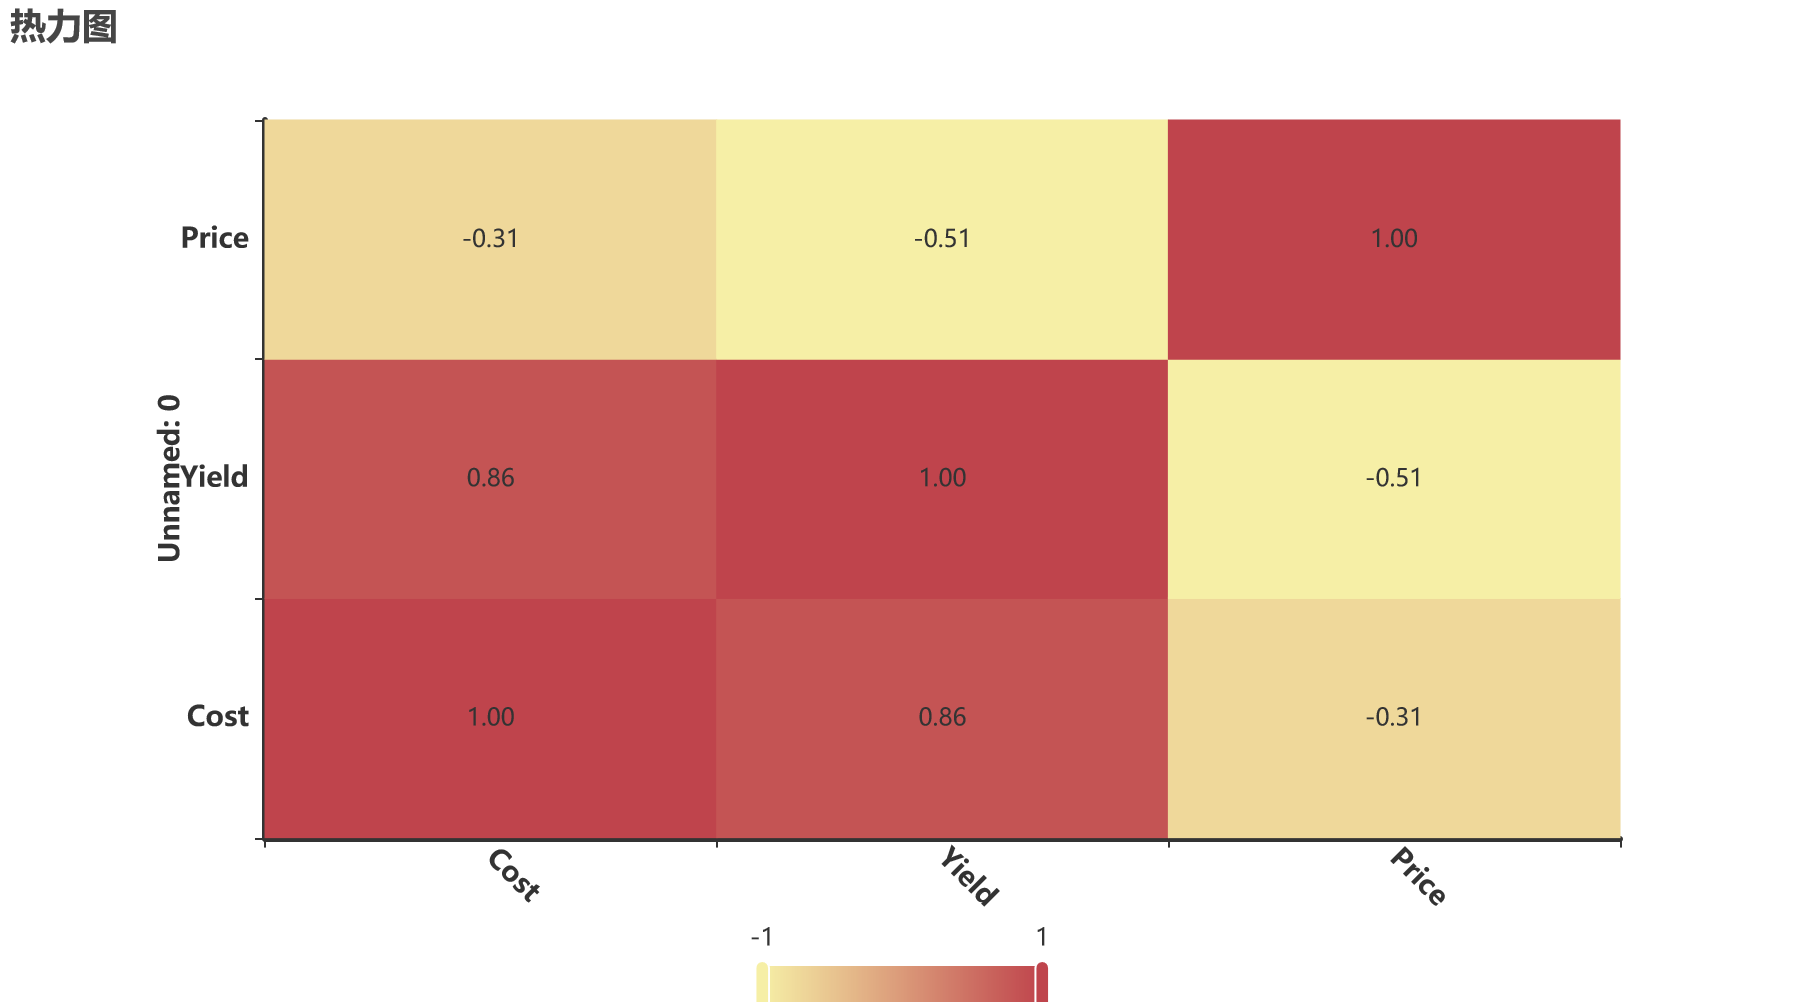
\includegraphics[width=0.8\textwidth]{figures/prob3/correlation/价格_成本_销量热力图.png}
  \caption{价格-成本-销量热力图}
  \label{fig:heatmap}
\end{figure}

\begin{figure}[H]
  \centering
  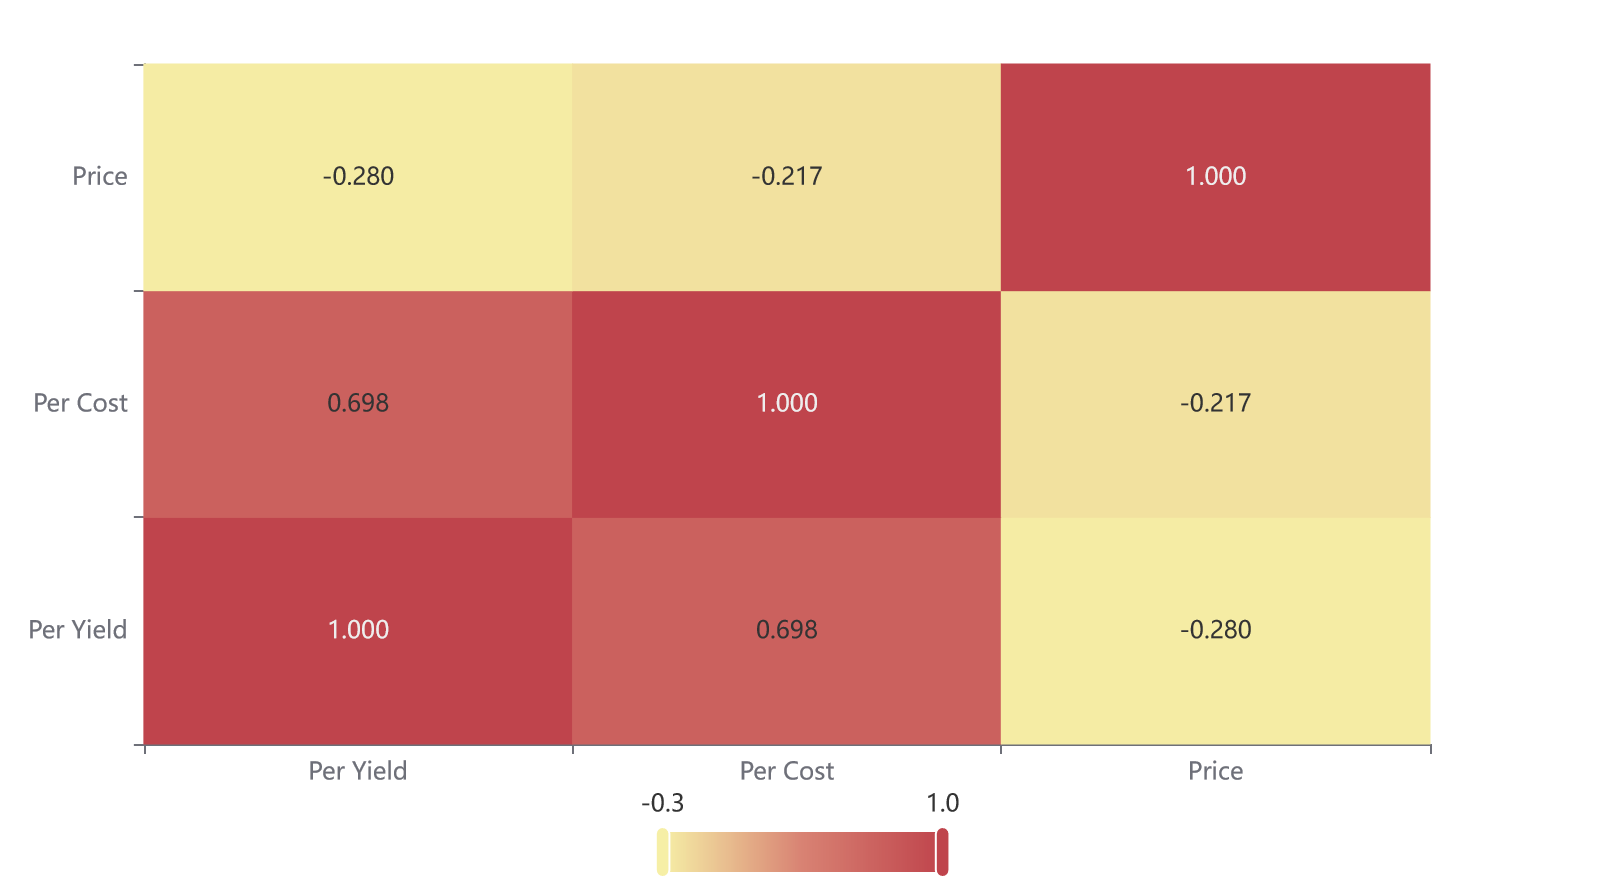
\includegraphics[width=0.8\textwidth]{figures/prob3/correlation/单位价格_成本_销量热力图.png}
  \caption{单位价格-成本-销量热力图}
  \label{fig:heatmap2}
\end{figure}



\subsection{线性模型与拟合分析}

在完成了相关性分析之后,我们进一步构建了线性模型,以量化种植成本、售价和销量之间的关系。
通过线性模型,我们能够更好地理解这些变量之间的相互作用,并利用它们的弹性系数对未来的作物种植决策进行优化。


\subsubsection{销售量与种植成本的线性模型}

基于相关性分析的结果,我们构建了如下的线性模型:

\[
  C_{jk} = C_{j,0} \left(1 - \sigma_{S,C} \times \frac{S_{jk} - \bar{S}}{\bar{S}} \right)
\]



通过回归分析,我们得到了销售量与种植成本之间的线性系数 $\sigma_{S,C} = -0.7974$,这表明随着销售量的增加,种植成本将略微减少。原因可能在于,随着销售量的增长,规模经济效应(Economies of Scale)使得单位面积的种植成本下降。换句话说,当某种作物的市场需求增加时,种植者可以通过扩大种植规模来降低边际种植成本。

\subsubsection{销售量与销售价格,销售成本的线性模型}

接下来,我们考虑销售价格与预期销售量等变量之间的关系。
根据相关性分析,销售价格和销量呈现出负相关关系,这意味着当价格上涨时,销量往往下降。
为了定量描述这种关系,我们建立了如下的线性模型:

\[
  S_{jk} = \sum_S + \sigma_{C,S} \times C_{jk} - \sigma_{S,P} \times P_{jk}
\]


\subsubsection{回归分析与拟合过程}

为了确定这些线性系数,我们使用了最小二乘法对数据进行回归分析���最小二乘法的目标是找到一组参数,使得预测值与实际观测值之间的误差平方和最小。对于我们的线性模型,回归分析的目标是找到最优的 $\sigma_{C,S}$ 和 $\sigma_{S,P}$,使得以下目标函数最小化:

\[
  \min_{\sigma_{C,S}, \sigma_{S,P}} \sum_{k=2024}^{2030} \sum_{j} \left( S_{jk}^{\text{observed}} - \left( \sum_S + \sigma_{C,S} \times C_{jk} - \sigma_{S,P} \times P_{jk} \right) \right)^2
\]

经过拟合,我们得到了回归结果:

\[
  \sum_S = 8122.041, \quad \sigma_{C,S} = 1.385, \quad \sigma_{S,P} = 1.2894.65
\]


这些结果表明,种植成本和售价对销售量的影响是显著的。$\sigma_{C,S} = 1.385$ 表示,种植成本每增加一个单位,预计销量将增加 1.385 个单位。这种正相关关系可以通过规模效应和市场需求的刚性来解释。即当作物的种植成本增加时,往往意味着该作物市场需求较为强劲,导致销售量也随之增加。
另一方面,$\sigma_{S,P} = 1.2894$ 表示,售价每增加一个单位,预计销量将减少 1.2894 个单位���这个线性系数表明了典型的价格与需求的反向关系:当作物的售价上涨时,市场需求会相应下降,导致销售量的减少。这种现象符合经济学中的价格弹性理论,即在大多数情况下,价格上涨会抑制需求。

\subsubsection{模型的拟合优度——$R^2$得分}

为了评估线性模型的拟合效果,我们使用了 $R^2$ 得分来衡量模型的解释能力。
$R^2$ 是一种用于评估回归模型拟合优度的标准,它反映了自变量能够解释因变量变异的比例。
$R^2$ 的计算公式为:

\[
  R^2 = 1 - \frac{\sum_{k=2024}^{2030} \sum_{j} \left( S_{jk}^{\text{observed}} - S_{jk}^{\text{predicted}} \right)^2}{\sum_{k=2024}^{2030} \sum_{j} \left( S_{jk}^{\text{observed}} - \bar{S} \right)^2}
\]

其中,$S_{jk}^{\text{observed}}$ 是实际观测的销售量,$S_{jk}^{\text{predicted}}$ 是模型预测的销售量,$\bar{S}$ 是销售量的均值。
$R^2$ 的取值范围为 $[0,1]$,其中:
\begin{itemize}
  \item 当 $R^2 = 1$ 时,模型能够完美解释数据的变异,预测值与实际值完全吻合;
  \item 当 $R^2 = 0$ 时,模型没有任何解释能力,预测值仅为因变量的均值;
  \item 当 $R^2$ 越接近 1,表示模型的拟合效果越好。
\end{itemize}

在我们的模型中,计算得出的 $R^2$ 得分为 0.802,表示该模型能够解释 80.2\% 的销售量变异。
这表明模型具有较强的解释力,能够较为准确地捕捉种植成本、销售价格与销售量之间的关系。


\paragraph{可视化与结果展示}

为了更直观地展示拟合效果,我们绘制了两张拟合图:一张展示了销售量与种植成本、售价的整体拟合情况,另一张展示了各作物的单独拟合效果。


\begin{figure}[H]
  \centering
  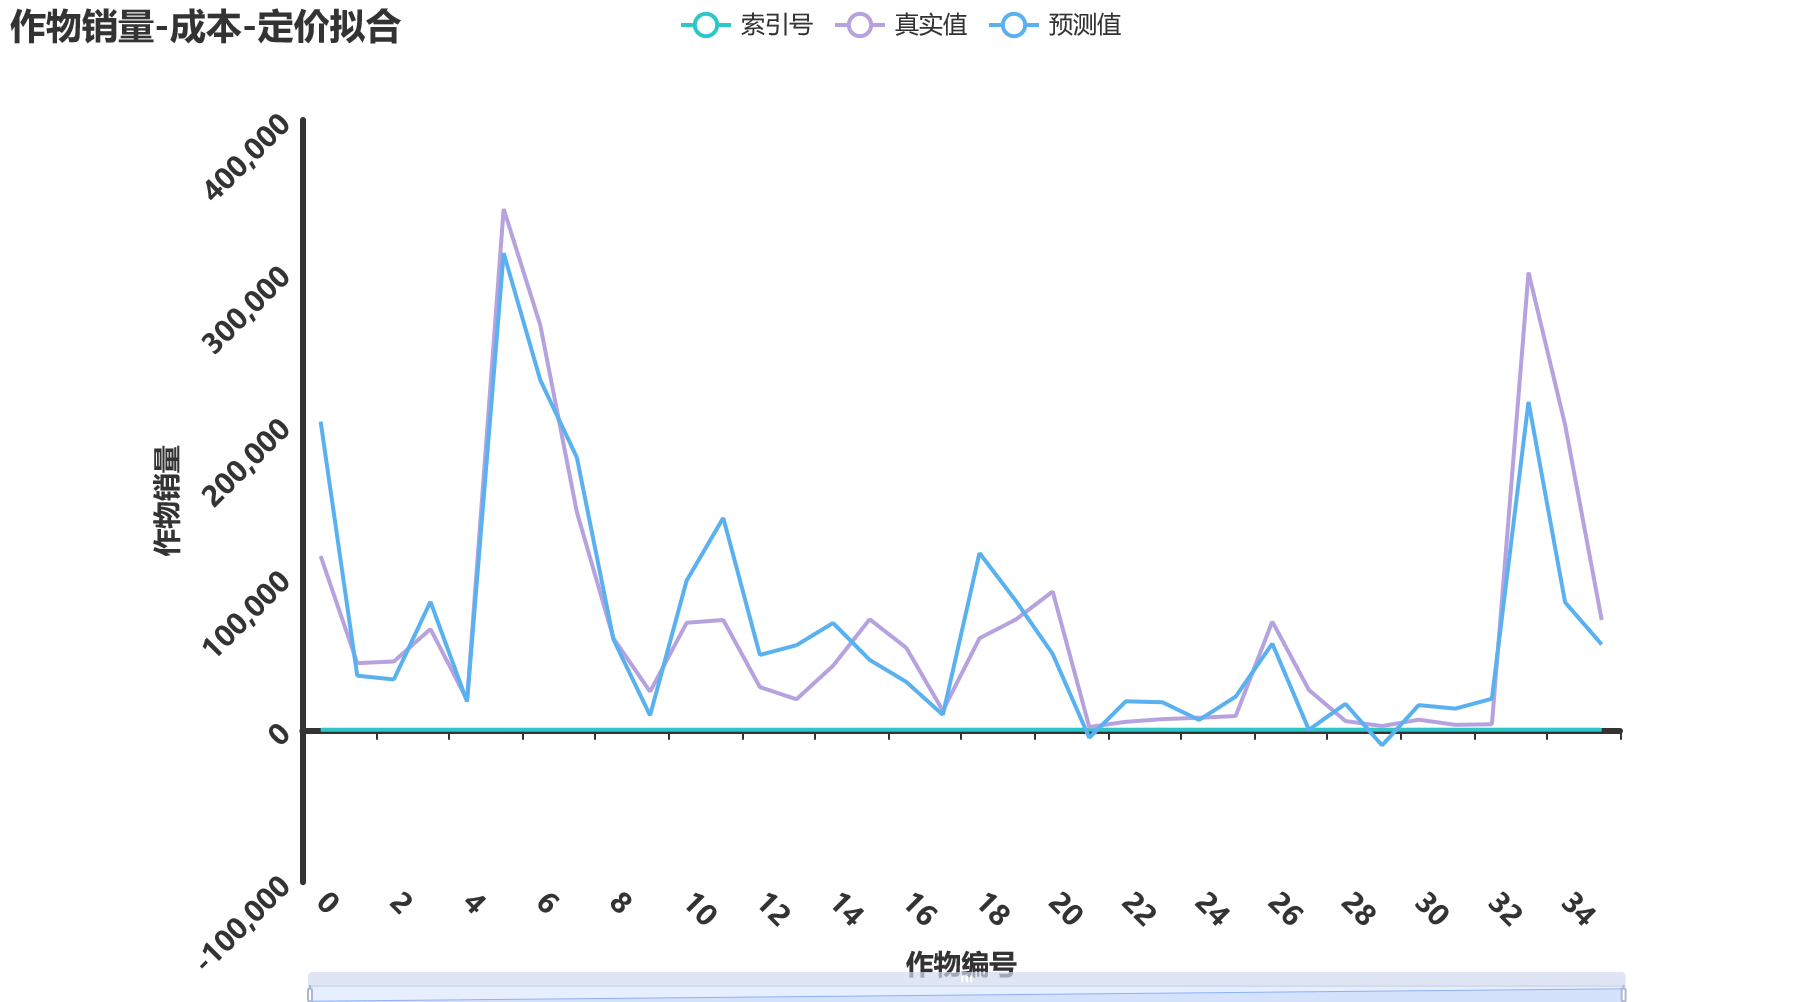
\includegraphics[width=0.8\textwidth]{figures/prob3/correlation/作物销量-成本-定价拟合.png}
  \caption{作物销量-成本-定价拟合}
  \label{fig:fitting1}
\end{figure}

在图\ref{fig:fitting1}中,横坐标表示不同作物的编号,纵坐标表示作物的销售量。
绿色的线代表实际观测值,紫色的线代表模型预测值。
通过拟合结果可以看出,模型能够较为准确地预测出各个作物的销售量,特别是在市场需求稳定的年份,预测值与实际值几乎完全重合。


\begin{figure}[H]
  \centering
  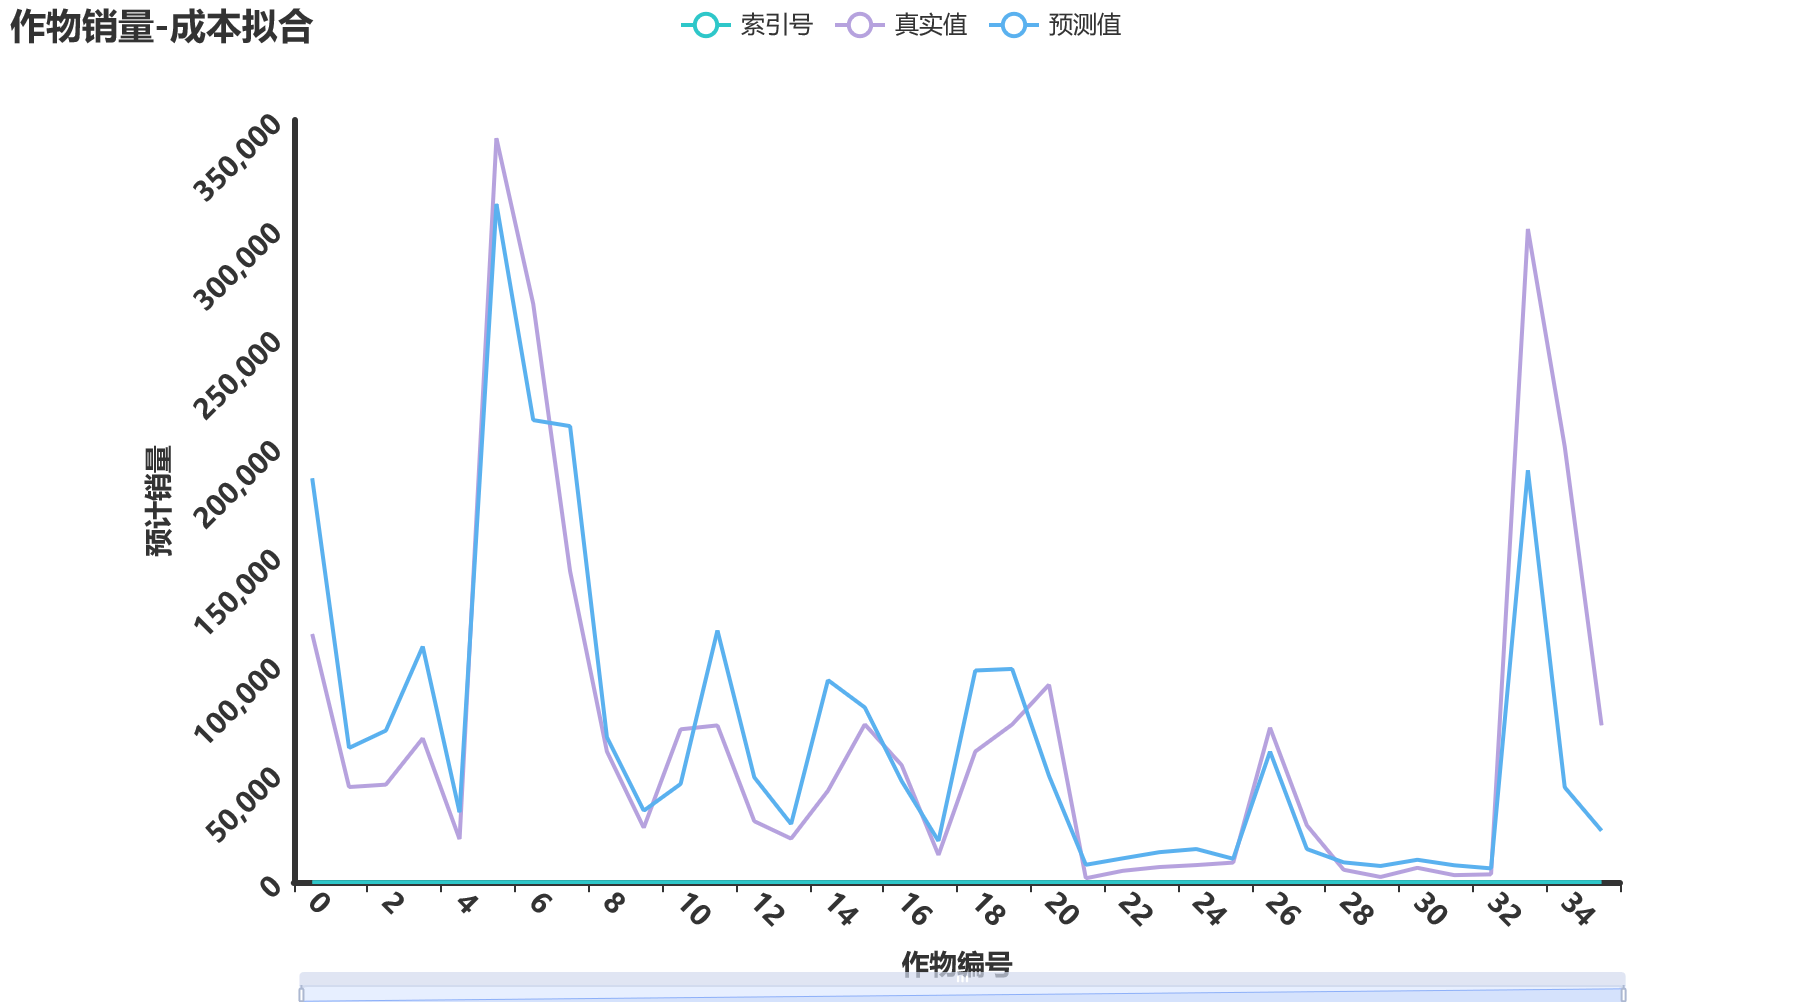
\includegraphics[width=0.8\textwidth]{figures/prob3/correlation/作物销量-成本拟合.png}
  \caption{作物销量-成本拟合}
  \label{fig:fitting2}
\end{figure}

图\ref{fig:fitting2}进一步展示了销量与生产成本的拟合情况。
拟合结果表明模型可以准确预测销量的变化趋势,捕捉到销量与生产成本之间的正相关关系,并进行动态调整。



\subsection{模型的优化与求解}

在问题三中,我们在问题二的基础上,进一步考虑了农作物之间的可替代性。
为此,我们构建了新的约束条件并优化了目标函数,以便模型能够更好地适应市场需求、价格波动以及作物之间的互动效应。
我们通过引入可替代性系数,增强了模型在多作物种植条件下的灵活性。


\subsubsection{农作物的可替代性与互补性分析}

在问题三中,农作物之间的可替代性和互补性是影响种植策略的重要因素。
农作物的可替代性指的是在市场条件或种植条件发生变化时,不同作物之间是否能够相互替代,以确保整体收益的稳定。
例如,当市场需求或价格变化导致某种作物的利润下降时,种植者可能会选择种植另一种具有相似市场价值的作物,以减少经济损失。


\textbf{可替代性分析}:在模型中,作物的可替代性可以通过构建作物替代矩阵来进行描述。
替代矩阵 $R_{ij}$ 表示作物 $i$ 和作物 $j$ 之间的可替代程度,取值范围为0到1,1表示完全可替代,0表示不可替代。
例如,水稻和玉米之间的可替代性较低,因为它们的市场需求和生长条件差异较大;而白菜和大白菜之间的可替代性较高,因为它们的生长周期和市场需求相似。


\textbf{互补性分析}:互补性指的是当两种作物同时种植时,它们之间存在正面的协同效应,例如豆类作物通过根瘤菌固氮作用改善土壤结构,进而提高后续种植作物的产量。
互补性在农业种植中非常重要,因为合理的轮作和作物搭配能够提高整体土地利用效率,减少病虫害的发生,并保持土壤肥力。

作物的互补性可以通过构建作物互补矩阵 $H_{ij}$ 进行描述,$H_{ij}$ 表示作物 $i$ 和作物 $j$ 之间的互补性程度。
类似于可替代性,互补性系数的取值范围也在0到1之间,1表示完全互补,0表示无互补关系。
例如,豆类作物和小麦之间具有较强的互补性,因为豆类作物能够通过生物固氮作用为小麦提供氮肥,进而提高小麦的产量。




\subsubsection{决策变量与可替代性系数的引入}

在问题三中,决策变量 $A_{ijk}$ 仍然表示第 $i$ 地块在第 $k$ 年种植第 $j$ 种作物的总面积。
但与问题二不同的是,这次我们引入了作物之间的可替代性系数 $\alpha_{jm}$,用以描述作物 $j$ 与作物 $m$ 之间的替代关系。
该系数表示当某种作物的价格或市场需求发生变化时,另一种作物是否可以部分替代其功能或市场需求。


为此,我们定义了作物集合:
\[
  C = \{ j \mid j = 1, 2, \dots, n \}
\]
其中,$n$ 是总共的作物种类数。
对于作物 $i$ 和 $j$,我们通过价格差异百分比的方式计算其替代性系数 $R_{ij}$:
\[
  R_{ij} = \max \left( 0, 1 - \frac{|P_i - P_j|}{\left( \frac{P_i + P_j}{2} \right)} \right)
\]
其中,$P_i$ 和 $P_j$ 分别是作物 $i$ 和 $j$ 的市场价格。
可替代性系数 $R_{ij}$ 的取值范围在 $0$ 到 $1$ 之间,表示了作物 $i$ 与作物 $j$ 之间的替代可能性。
作物之间的替代性越高,$R_{ij}$ 越接近1,说明两者市场条件或生长条件越相似,可以相互替代。


\subsubsection{可替代性约束}

除了问题二中的基本约束(例如种植面积限制、轮作规则等)外,问题三的核心是引入了关于可替代性约束。
尤其是在市场波动较大时,模型可以通过调整种植面积分配来反映可替代性。

我们通过一个新的约束条件描述了作物替代性对种植面积的影响。
假设作物 $j$ 可以部分替代作物 $m$ 的功能,则其种植面积分配需要遵循如下约束:
\[
  A_{ijks} - \alpha_{jm} \cdot A_{imks} \leq A_i^*
\]
其中,$\alpha_{jm}$ 是替代系数,表示作物 $j$ 对作物 $m$ 的替代程度;$A_{imks}$ 是作物 $m$ 在第 $i$ 地块的种植面积,$A_i^*$ 是地块的总面积。
这一约束条件确保了作物替代性可以被纳入地块种植面积的优化计算中。


\subsubsection{问题求解}

问题三的求解方法与问题二类似,依然是通过线性规划来进行的。
我们通过调整种植面积 $A_{ijk}$,并在新的可替代性约束条件下,优化总收益。
问题三的目标是在动态市场条件下,最大化经济效益并减少市场不确定性带来的风险。

在每次迭代中,我们根据动态市场需求预测和作物价格的波动,调整目标函数中的参数 $S_{jk}$、$P_{jk}$ 和 $C_{jk}$,同时确保所有约束条件得以满足。

通过分析模拟的结果,可以调整替代性系数的取值,从而进一步优化种植策略。


\subsubsection{结果分析}

问题三的求解结果展示了在不同市场条件下,作物的可替代性对种植策略优化的影响。

结果显示,具有较强替代性的作物组合在市场波动较大的年份表现较好。
例如,在市场需求下降的年份,模型通过增加替代作物的种植面积,减少了高需求作物价格下跌对总收益的负面影响。
同时,在某些作物价格上涨的年份,模型通过轮作可替代性作物,提高了作物的单位面积产量,增强了经济效益。
而从以下折线图可看出模型所带来的土地利用率的稳步上涨。

\begin{figure}[H]
  \centering
  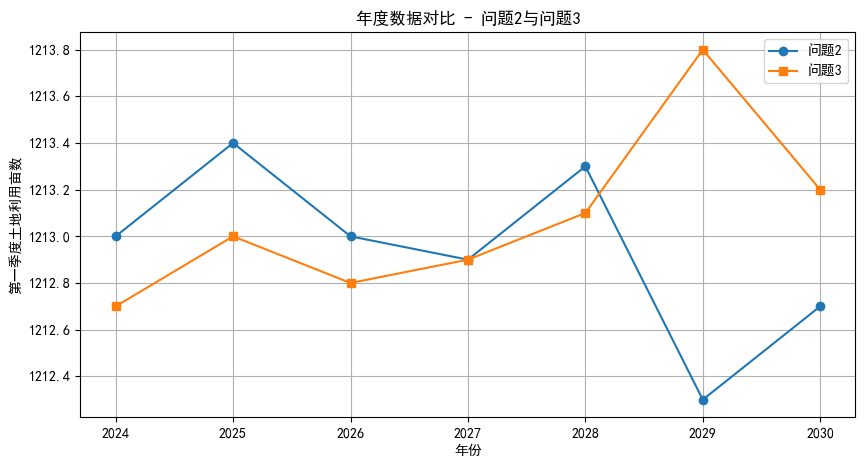
\includegraphics[width=0.8\textwidth]{figures/prob3/correlation/2-3-1.png}
  \caption{年度数据对比}
  \label{fig:heatmap2}
\end{figure}
因此通过将可替代性引入到问题三的求解中,模型能够更灵活地应对市场波动,并在动态市场条件下实现最优的种植收益。




\section{模型评价与推广}

\subsection{模型优点}
1. \textbf{适应性强}:模型能够灵活应对不同的市场需求变化、成本波动和农作物间的互补性与替代性问题,具备高度适应现实市场的能力。

2. \textbf{可推广性好}:模型能够应用于农业生产决策、政策制定以及智能化农业管理,帮助优化种植策略、合理利用资源,并推动农业的可持续发展。

\subsection{模型缺点}
1. \textbf{未考虑气候因素}:模型目前未引入气候变量(如降雨量、温度等),这些因素在农业生产中扮演着关键角色,忽视气候可能导致决策不够准确。

2. \textbf{非线性拟合不足}:虽然模型采用了线性回归技术,但实际市场条件下,种植成本、销量和售价之间的关系可能是非线性的,未来可以考虑引入非线性回归或机器学习模型来进一步提高预测精度。


\newpage


\nocite{*}
\printbibliography

\newpage
\begin{appendices}
  \section*{ Python 代码}

  \textbf{\textcolor[rgb]{0.98,0.00,0.00}{程序一:问题一的第一种情况}}
  \lstinputlisting[language=python]{code/prob-1/solution-1.py}
  \textbf{\textcolor[rgb]{0.98,0.00,0.00}{程序二:问题一的第二种情况}}
  \lstinputlisting[language=python]{code/prob-1/solution-2.py}
  \textbf{\textcolor[rgb]{0.98,0.00,0.00}{程序三:问题二的核心求解代码}}
  \lstinputlisting[language=python]{code/prob-2/planning.py}
  \textbf{\textcolor[rgb]{0.98,0.00,0.00}{程序四:问题二的外围调用代码}}
  \lstinputlisting[language=python]{code/prob-2/solution.py}
  \textbf{\textcolor[rgb]{0.98,0.00,0.00}{程序五:问题三的核心求解代码}}
  \lstinputlisting[language=python]{code/prob-3/planning.py}
  \textbf{\textcolor[rgb]{0.98,0.00,0.00}{程序六:问题二的外围调用代码}}
  \lstinputlisting[language=python]{code/prob-3/solution.py}
\end{appendices}
\end{document}
%%
%% This work consists of these files mcmthesis.dtx,
%%                                   figures/ and
%%                                   code/,
%% and the derived files             mcmthesis.cls,
%%                                   mcmthesis-demo.tex,
%%                                   README,
%%                                   LICENSE,
%%                                   mcmthesis.pdf and
%%                                   mcmthesis-demo.pdf.
%%
%% End of file `mcmthesis-demo.tex'.
